% Options for packages loaded elsewhere
\PassOptionsToPackage{unicode}{hyperref}
\PassOptionsToPackage{hyphens}{url}
%
\documentclass[
]{article}
\usepackage{amsmath,amssymb}
\usepackage{iftex}
\ifPDFTeX
  \usepackage[T1]{fontenc}
  \usepackage[utf8]{inputenc}
  \usepackage{textcomp} % provide euro and other symbols
\else % if luatex or xetex
  \usepackage{unicode-math} % this also loads fontspec
  \defaultfontfeatures{Scale=MatchLowercase}
  \defaultfontfeatures[\rmfamily]{Ligatures=TeX,Scale=1}
\fi
\usepackage{lmodern}
\ifPDFTeX\else
  % xetex/luatex font selection
\fi
% Use upquote if available, for straight quotes in verbatim environments
\IfFileExists{upquote.sty}{\usepackage{upquote}}{}
\IfFileExists{microtype.sty}{% use microtype if available
  \usepackage[]{microtype}
  \UseMicrotypeSet[protrusion]{basicmath} % disable protrusion for tt fonts
}{}
\makeatletter
\@ifundefined{KOMAClassName}{% if non-KOMA class
  \IfFileExists{parskip.sty}{%
    \usepackage{parskip}
  }{% else
    \setlength{\parindent}{0pt}
    \setlength{\parskip}{6pt plus 2pt minus 1pt}}
}{% if KOMA class
  \KOMAoptions{parskip=half}}
\makeatother
\usepackage{xcolor}
\usepackage[margin=1in]{geometry}
\usepackage{color}
\usepackage{fancyvrb}
\newcommand{\VerbBar}{|}
\newcommand{\VERB}{\Verb[commandchars=\\\{\}]}
\DefineVerbatimEnvironment{Highlighting}{Verbatim}{commandchars=\\\{\}}
% Add ',fontsize=\small' for more characters per line
\usepackage{framed}
\definecolor{shadecolor}{RGB}{248,248,248}
\newenvironment{Shaded}{\begin{snugshade}}{\end{snugshade}}
\newcommand{\AlertTok}[1]{\textcolor[rgb]{0.94,0.16,0.16}{#1}}
\newcommand{\AnnotationTok}[1]{\textcolor[rgb]{0.56,0.35,0.01}{\textbf{\textit{#1}}}}
\newcommand{\AttributeTok}[1]{\textcolor[rgb]{0.13,0.29,0.53}{#1}}
\newcommand{\BaseNTok}[1]{\textcolor[rgb]{0.00,0.00,0.81}{#1}}
\newcommand{\BuiltInTok}[1]{#1}
\newcommand{\CharTok}[1]{\textcolor[rgb]{0.31,0.60,0.02}{#1}}
\newcommand{\CommentTok}[1]{\textcolor[rgb]{0.56,0.35,0.01}{\textit{#1}}}
\newcommand{\CommentVarTok}[1]{\textcolor[rgb]{0.56,0.35,0.01}{\textbf{\textit{#1}}}}
\newcommand{\ConstantTok}[1]{\textcolor[rgb]{0.56,0.35,0.01}{#1}}
\newcommand{\ControlFlowTok}[1]{\textcolor[rgb]{0.13,0.29,0.53}{\textbf{#1}}}
\newcommand{\DataTypeTok}[1]{\textcolor[rgb]{0.13,0.29,0.53}{#1}}
\newcommand{\DecValTok}[1]{\textcolor[rgb]{0.00,0.00,0.81}{#1}}
\newcommand{\DocumentationTok}[1]{\textcolor[rgb]{0.56,0.35,0.01}{\textbf{\textit{#1}}}}
\newcommand{\ErrorTok}[1]{\textcolor[rgb]{0.64,0.00,0.00}{\textbf{#1}}}
\newcommand{\ExtensionTok}[1]{#1}
\newcommand{\FloatTok}[1]{\textcolor[rgb]{0.00,0.00,0.81}{#1}}
\newcommand{\FunctionTok}[1]{\textcolor[rgb]{0.13,0.29,0.53}{\textbf{#1}}}
\newcommand{\ImportTok}[1]{#1}
\newcommand{\InformationTok}[1]{\textcolor[rgb]{0.56,0.35,0.01}{\textbf{\textit{#1}}}}
\newcommand{\KeywordTok}[1]{\textcolor[rgb]{0.13,0.29,0.53}{\textbf{#1}}}
\newcommand{\NormalTok}[1]{#1}
\newcommand{\OperatorTok}[1]{\textcolor[rgb]{0.81,0.36,0.00}{\textbf{#1}}}
\newcommand{\OtherTok}[1]{\textcolor[rgb]{0.56,0.35,0.01}{#1}}
\newcommand{\PreprocessorTok}[1]{\textcolor[rgb]{0.56,0.35,0.01}{\textit{#1}}}
\newcommand{\RegionMarkerTok}[1]{#1}
\newcommand{\SpecialCharTok}[1]{\textcolor[rgb]{0.81,0.36,0.00}{\textbf{#1}}}
\newcommand{\SpecialStringTok}[1]{\textcolor[rgb]{0.31,0.60,0.02}{#1}}
\newcommand{\StringTok}[1]{\textcolor[rgb]{0.31,0.60,0.02}{#1}}
\newcommand{\VariableTok}[1]{\textcolor[rgb]{0.00,0.00,0.00}{#1}}
\newcommand{\VerbatimStringTok}[1]{\textcolor[rgb]{0.31,0.60,0.02}{#1}}
\newcommand{\WarningTok}[1]{\textcolor[rgb]{0.56,0.35,0.01}{\textbf{\textit{#1}}}}
\usepackage{longtable,booktabs,array}
\usepackage{calc} % for calculating minipage widths
% Correct order of tables after \paragraph or \subparagraph
\usepackage{etoolbox}
\makeatletter
\patchcmd\longtable{\par}{\if@noskipsec\mbox{}\fi\par}{}{}
\makeatother
% Allow footnotes in longtable head/foot
\IfFileExists{footnotehyper.sty}{\usepackage{footnotehyper}}{\usepackage{footnote}}
\makesavenoteenv{longtable}
\usepackage{graphicx}
\makeatletter
\def\maxwidth{\ifdim\Gin@nat@width>\linewidth\linewidth\else\Gin@nat@width\fi}
\def\maxheight{\ifdim\Gin@nat@height>\textheight\textheight\else\Gin@nat@height\fi}
\makeatother
% Scale images if necessary, so that they will not overflow the page
% margins by default, and it is still possible to overwrite the defaults
% using explicit options in \includegraphics[width, height, ...]{}
\setkeys{Gin}{width=\maxwidth,height=\maxheight,keepaspectratio}
% Set default figure placement to htbp
\makeatletter
\def\fps@figure{htbp}
\makeatother
\setlength{\emergencystretch}{3em} % prevent overfull lines
\providecommand{\tightlist}{%
  \setlength{\itemsep}{0pt}\setlength{\parskip}{0pt}}
\setcounter{secnumdepth}{5}
\usepackage{booktabs}
\usepackage{longtable}
\usepackage{array}
\usepackage{multirow}
\usepackage{wrapfig}
\usepackage{float}
\usepackage{colortbl}
\usepackage{pdflscape}
\usepackage{tabu}
\usepackage{threeparttable}
\usepackage{threeparttablex}
\usepackage[normalem]{ulem}
\usepackage{makecell}
\usepackage{xcolor}
\ifLuaTeX
  \usepackage{selnolig}  % disable illegal ligatures
\fi
\usepackage{bookmark}
\IfFileExists{xurl.sty}{\usepackage{xurl}}{} % add URL line breaks if available
\urlstyle{same}
\hypersetup{
  pdftitle={Análisis de datos ómicos - PEC 1},
  pdfauthor={Liliana Cifuentes},
  hidelinks,
  pdfcreator={LaTeX via pandoc}}

\title{Análisis de datos ómicos - PEC 1}
\author{Liliana Cifuentes}
\date{}

\begin{document}
\maketitle

{
\setcounter{tocdepth}{2}
\tableofcontents
}
\section{Resumen}\label{resumen}

El síndrome metabólico de la caquexia es una condición importante en la
salud pública al implicar catabolismo tisular, que se asocia a
discapacidad y bajas tasas de supervivencia en los pacientes con una
enfermedad subyacente. El \texttt{dataset} \texttt{human\_cachexia}
proporciona datos metabolómicos relevantes, pacientes con cáncer de
colon o pulmón, con o sin el síndrome, que a través de un análisis y
estudio de los mismos permite identificar las alteraciones y patrones en
los metabolitos involucrados en el catabolismo muscular. Se implementó
\texttt{SummarizedExperiment} por su flexibilidad y utilidad en el uso
de datos experimentales, a través del cual se realizaron análisis
descriptivos de los datos, encontrando que aquellos metabolitos
vinculados con la pérdida muscular, tales como la Creatinina, la Glucosa
y aquellos pertenecientes a las vías del metabolismo de aminoácidos,
presentan variabilidades destacables, con tendencias a niveles mayores.

\begin{center}\rule{0.5\linewidth}{0.5pt}\end{center}

\section{Objetivos}\label{objetivos}

\begin{itemize}
\item
  Desarrollar habilidades en el manejo de GitHub y su integración con un
  proyecto en R, para la gestión de versiones.
\item
  Analizar las diferencias clave entre las clases \texttt{ExpressionSet}
  y \texttt{SummarizedExperiment} del proyecto \texttt{Bioconductor},
  para aplicarlo en el análisis de datos ómicos.
\item
  Realizar un análisis exploratorio del \texttt{dataset} metabolómico
  \texttt{human\_cachexia}, a partir de la clase
  \texttt{SummarizedExperiment}, con el fin de identificar patrones y
  relaciones relevantes entre las variables, para obtener una
  comprensión de los datos en el contexto de estudios sobre caquexia y
  la vía metabólica del catabolismo muscular en pacientes con cáncer.
\end{itemize}

\begin{center}\rule{0.5\linewidth}{0.5pt}\end{center}

\section{Métodos}\label{muxe9todos}

Se creó un repositorio en GitHub para la gestión de versiones. Se
seleccionó el \texttt{dataset} \texttt{human\_cachexia} por su
relevancia en salud pública, y se leyó directamente, desde el
repositorio \texttt{nutrimetabolomics} en GitHub, en lenguaje de
programación R. Posteriormente, se creó la clase
\texttt{SummarizedExperiment} a través de R, almacenando los datos de
expresión de los metabolitos, los metadatos de los metabolitos, los
metadatos de las muestras en el atributo correspondiente para cada uno
de estos, y creando el atributo \texttt{metadata} con la información
disponible en el artículo de Eisner et al., 2010 desde donde se
extrajeron los datos del \texttt{dataset}.

Se realizó un análisis exploratorio de los datos, evaluando inicialmente
la estructura de la base de datos y sus metadatos a través de los
atributos assay, colData y rowData, verificando a su vez la ausencia de
datos con las funciones sum e is.nan. Asimismo, se calculó un resumen
estadístico por metabolito a través de la función summary. A partir de
lo observado en este análisis, se calcularon las diferencias entre las
medias y las medianas de los niveles de los metabolitos con el fin de
verificar la simetría en la distribución de las muestras. También, se
evaluó la variabilidad de los niveles de los metabolitos a través del
cálculo de la desviación estándar para cada metabolito y se graficó en
un diagrama de barras.

Se obtuvo un mapa de calor directamente de la matriz correspondiente a
los niveles de los metabolitos, buscando identificar patrones en los
mismos, y de igual forma se calculó la matriz de correlación entre los
metabolitos, la cual fue visualizada a través de un mapa de calor; estos
mapas se obtuvieron a través de la función pheatmap. Finalmente, se
realizó un análisis de componentes principales (PCA) a través de la
función prcomp, con el cual se redujo la dimensionalidad de la base de
datos, y se pudieron identificar diferencias en la variabilidad de los
datos de acuerdo con el grupo de pacientes (cachexia o control) o las
categorías a las cuales se podían asociar los metabolitos de acuerdo con
la literatura relacionada con las vías metabólicas, obtenida a partir de
(METACYC, 2025).

\begin{center}\rule{0.5\linewidth}{0.5pt}\end{center}

\section{Resultados}\label{resultados}

El \texttt{dataset} \texttt{human\_cachexia} fue seleccionado debido a
se trata de una base de datos públicamente disponible a través del
repositorio \texttt{nutrimetabolomics} en GitHub de Sánchez Pla, A.; lo
que permite su exploración y utilización. La información del
Data\_Catalog, en el mismo repositorio, describe que posee con 77
muestras de orina (47 pacientes con caquexia y 30 pacientes control) y
63 características; y dentro de su descripción se garantiza que las
muestras no están emparejadas, que todos los valores de los datos son
numéricos, y se detectaron 0 valores faltantes; lo que sugiere que se
trata de una base de datos con buena calidad.

Esta base de datos se relaciona con un síndrome metabólico complejo,
incapacitante y potencialmente mortal: la caquexia, que está asociada a
enfermedades crónicas, como el cáncer, EPOC, CHF, etc.; y se caracteriza
por alteraciones en el metabolismo que implican catabolismo tisular
(pérdida de masa muscular), lo cual se traduce en pérdida de peso,
fuerza y fatiga extrema. Este síndrome al estar relacionado con una
enfermedad subyacente tiene un impacto significativo en el paciente al
afectar la tolerancia hacia el tratamiento, ya que se asocia a la
discapacidad y a bajas tasas de supervivencia, lo que la convierte en
una condición relevante en la salud pública. Actualmente se cuenta con
ciertos tratamientos, como la suplementación nutricional, sin embargo,
estos no son capaces de ralentizar el metabolismo o revertir el síndrome
(Pfizer, 2025)

Por lo tanto, esta base de datos metabolómicos en caquexia que incluye
pacientes con cáncer de colon o pulmón, con o sin perdida muscular, a
los cuales se les realizó un estudio de orina para identificar varios
metabolitos excretados e involucrados en el catabolismo muscular, y por
lo tanto relacionados con este síndrome (Eisner, R. et al, 2010),
permitiría identificar alteraciones y patrones de dichos metabolitos;
con el fin de comprender esta relación y como punto de partida para
posteriores investigaciones que contribuyan a establecer tratamientos
eficaces.

Para leer el \texttt{dataset} de metabolómica \texttt{human\_cachexia},
del repositorio de GitHub proporcionado, se realizarón los siguientes
pasos:

\begin{Shaded}
\begin{Highlighting}[]
\CommentTok{\# Instalar paquete}
\CommentTok{\#install.packages("readr")}

\CommentTok{\# Llamar librerias}
\FunctionTok{library}\NormalTok{(readr)}
\FunctionTok{library}\NormalTok{(knitr)}

\CommentTok{\# Definir la URL del archivo}
\NormalTok{url }\OtherTok{=} \StringTok{"https://raw.githubusercontent.com/nutrimetabolomics/metaboData/refs/heads/main/Datasets/2024{-}Cachexia/human\_cachexia.csv"}

\CommentTok{\# Leer el archivo CSV}
\NormalTok{data }\OtherTok{=} \FunctionTok{read\_csv}\NormalTok{(url)}
\end{Highlighting}
\end{Shaded}

\begin{verbatim}
## Rows: 77 Columns: 65
## -- Column specification --------------------------------------------------------
## Delimiter: ","
## chr  (2): Patient ID, Muscle loss
## dbl (63): 1,6-Anhydro-beta-D-glucose, 1-Methylnicotinamide, 2-Aminobutyrate,...
## 
## i Use `spec()` to retrieve the full column specification for this data.
## i Specify the column types or set `show_col_types = FALSE` to quiet this message.
\end{verbatim}

Con la lectura del data frame se visualiza que se trata de una tabla con
77 filas y 65 columnas, con 2 características formato caracter (Patient
ID, y Muscle loss) y 63 formato numerico. Luego, se creo el objeto clase
\texttt{SummarizedExperiment} como se explica en el siguiente código:

\begin{Shaded}
\begin{Highlighting}[]
\CommentTok{\# Instalar paquetes}
\CommentTok{\#install.packages("BiocManager")}
\CommentTok{\#BiocManager::install("SummarizedExperiment")}

\CommentTok{\# Llamar libreria}
\FunctionTok{library}\NormalTok{(SummarizedExperiment)}

\CommentTok{\# Crear clase SummarizedExperiment}

\CommentTok{\# Crear argumento assay (datos de expresion de metabolitos)}
\NormalTok{ensayo }\OtherTok{=} \FunctionTok{t}\NormalTok{(}\FunctionTok{as.matrix}\NormalTok{(data[,}\SpecialCharTok{!}\NormalTok{(}\FunctionTok{colnames}\NormalTok{(data) }\SpecialCharTok{\%in\%} \FunctionTok{c}\NormalTok{(}\StringTok{"Patient ID"}\NormalTok{, }\StringTok{"Muscle loss"}\NormalTok{))]))}
\FunctionTok{colnames}\NormalTok{(ensayo) }\OtherTok{=}\NormalTok{ data}\SpecialCharTok{$}\StringTok{\textasciigrave{}}\AttributeTok{Patient ID}\StringTok{\textasciigrave{}} \CommentTok{\# Asignar nombre}

\CommentTok{\# Crear argumento rowdata (metadatos de los metabolitos)}
\NormalTok{rowdata }\OtherTok{=} \FunctionTok{data.frame}\NormalTok{(}\AttributeTok{metabolito=}\FunctionTok{tail}\NormalTok{(}\FunctionTok{colnames}\NormalTok{(data),}\SpecialCharTok{{-}}\DecValTok{2}\NormalTok{))}

\CommentTok{\# Crear argumento coldata (metadatos de las muestras)}
\NormalTok{coldata }\OtherTok{=} \FunctionTok{data.frame}\NormalTok{(}\AttributeTok{grupo=}\NormalTok{data}\SpecialCharTok{$}\StringTok{\textasciigrave{}}\AttributeTok{Muscle loss}\StringTok{\textasciigrave{}}\NormalTok{, }\AttributeTok{row.names=}\NormalTok{data}\SpecialCharTok{$}\StringTok{\textasciigrave{}}\AttributeTok{Patient ID}\StringTok{\textasciigrave{}}\NormalTok{)}

\CommentTok{\# Añadir metadatos adicionales sobre el experimento}
\NormalTok{metadatos }\OtherTok{=} \FunctionTok{list}\NormalTok{(}\AttributeTok{experiment\_date =} \StringTok{"2010{-}08{-}01"}\NormalTok{, }\AttributeTok{protocol =} \StringTok{"detección de metabolitos en orina a través del espectrómetro de RMN Varian INOVA de 600 MHz, sonda de triple eje con gradiente de 5{-}mm HCN; e identificados a través del software Chenomx NMRSuite 4.6"}\NormalTok{, }\AttributeTok{researchers =} \StringTok{"Roman Eisner, Cynthia Stretch, Thomas Eastman, Jianguo Xia, David Hau, Sambasivarao Damaraju, Russell Greiner, David S. Wishart \& Vickie E. Baracos"}\NormalTok{, }\AttributeTok{study\_name =} \StringTok{"Learning to predict cancer{-}associated skeletal muscle wasting from 1H{-}NMR profiles of urinary metabolites"}\NormalTok{)}

\CommentTok{\# Crear SummarizedExperiment}
\NormalTok{experimento }\OtherTok{=} \FunctionTok{SummarizedExperiment}\NormalTok{(}\AttributeTok{assay=}\FunctionTok{list}\NormalTok{(}\AttributeTok{ensayo=}\NormalTok{ensayo), }\AttributeTok{rowData=}\NormalTok{rowdata, }\AttributeTok{colData=}\NormalTok{coldata, }\AttributeTok{metadata=}\NormalTok{metadatos)}

\CommentTok{\# Guardar en formato .Rda}
\FunctionTok{save}\NormalTok{(experimento, }\AttributeTok{file =} \StringTok{"SummarizedExperiment.Rda"}\NormalTok{)}
\end{Highlighting}
\end{Shaded}

A continuación, se realizó un análisis exploratorio general del objeto
clase \texttt{SummarizedExperiment} creado.

\begin{Shaded}
\begin{Highlighting}[]
\CommentTok{\# Instalar paquetes}
\CommentTok{\#install.packages("kableExtra")}

\CommentTok{\# Llamar librerias}
\FunctionTok{library}\NormalTok{(dplyr)}

\CommentTok{\# Definir tabla con la informacion del atributo metadata}
\NormalTok{infoDF }\OtherTok{=} \FunctionTok{data.frame}\NormalTok{(}\FunctionTok{matrix}\NormalTok{(}\FunctionTok{rep}\NormalTok{(}\ConstantTok{NA}\NormalTok{, }\DecValTok{2} \SpecialCharTok{*} \FunctionTok{length}\NormalTok{(metadatos)), }\AttributeTok{ncol =} \DecValTok{2}\NormalTok{))}
\ControlFlowTok{for}\NormalTok{ (i }\ControlFlowTok{in} \DecValTok{1}\SpecialCharTok{:}\FunctionTok{length}\NormalTok{(metadatos)) \{}
\NormalTok{    infoDF[i, }\DecValTok{1}\NormalTok{] }\OtherTok{=} \FunctionTok{names}\NormalTok{(metadatos)[i]}
\NormalTok{    infoDF[i, }\DecValTok{2}\NormalTok{] }\OtherTok{=}\NormalTok{ metadatos[i]}
\NormalTok{\}}
\FunctionTok{colnames}\NormalTok{(infoDF) }\OtherTok{=} \FunctionTok{c}\NormalTok{(}\StringTok{"Campo"}\NormalTok{, }\StringTok{"Descripción"}\NormalTok{)}

\CommentTok{\# Imprimir}
\NormalTok{infoDF }\SpecialCharTok{\%\textgreater{}\%}
\NormalTok{    kableExtra}\SpecialCharTok{::}\FunctionTok{kable}\NormalTok{() }\SpecialCharTok{\%\textgreater{}\%}
\NormalTok{    kableExtra}\SpecialCharTok{::}\FunctionTok{kable\_styling}\NormalTok{()}
\end{Highlighting}
\end{Shaded}

\begin{longtable}[t]{ll}
\toprule
Campo & Descripción\\
\midrule
experiment\_date & 2010-08-01\\
protocol & detección de metabolitos en orina a través del espectrómetro de RMN Varian INOVA de 600 MHz, sonda de triple eje con gradiente de 5-mm HCN; e identificados a través del software Chenomx NMRSuite 4.6\\
researchers & Roman Eisner, Cynthia Stretch, Thomas Eastman, Jianguo Xia, David Hau, Sambasivarao Damaraju, Russell Greiner, David S. Wishart \& Vickie E. Baracos\\
study\_name & Learning to predict cancer-associated skeletal muscle wasting from 1H-NMR profiles of urinary metabolites\\
\bottomrule
\end{longtable}

Se verificó que la clase estuviera estructurada correctamente
visualizando las primeras 6 características de la matriz \texttt{assay},
y las primeras y últimas 6 muestras con el respectivo grupo al que
pertenecen, y las primeras 6 características (metabolitos); encontrando
que se construyó correctamente (ver Anexo).

Se verificó que efectivamente la base de datos no tiene valores
faltantes:

\begin{Shaded}
\begin{Highlighting}[]
\CommentTok{\# Obtener el numero de valores faltantes en la matriz}
\FunctionTok{sum}\NormalTok{(}\FunctionTok{is.nan}\NormalTok{(}\FunctionTok{assay}\NormalTok{(experimento)))}
\end{Highlighting}
\end{Shaded}

\begin{verbatim}
## [1] 0
\end{verbatim}

Se realizó un resumen estadístico por metabolito con el fin de
identificar de forma más rápida si los valores encontrados en la muestra
en general, corresponden a los rangos esperados para cada metabolito;
encontrando que todos los metabolitos tienen valores mínimos y máximos
extremos.

\begin{Shaded}
\begin{Highlighting}[]
\CommentTok{\# Realizar resumen estadistico descriptivo de los datos por metabolito}
\FunctionTok{summary}\NormalTok{(}\FunctionTok{t}\NormalTok{(}\FunctionTok{assay}\NormalTok{(experimento)))}
\end{Highlighting}
\end{Shaded}

\begin{verbatim}
##  1,6-Anhydro-beta-D-glucose 1-Methylnicotinamide 2-Aminobutyrate 
##  Min.   :  4.71             Min.   :   6.42      Min.   :  1.28  
##  1st Qu.: 28.79             1st Qu.:  15.80      1st Qu.:  5.26  
##  Median : 45.60             Median :  36.60      Median : 10.49  
##  Mean   :105.63             Mean   :  71.57      Mean   : 18.16  
##  3rd Qu.:141.17             3rd Qu.:  73.70      3rd Qu.: 19.49  
##  Max.   :685.40             Max.   :1032.77      Max.   :172.43  
##  2-Hydroxyisobutyrate 2-Oxoglutarate    3-Aminoisobutyrate 3-Hydroxybutyrate
##  Min.   : 4.85        Min.   :   5.53   Min.   :   2.61    Min.   :  1.70   
##  1st Qu.:15.80        1st Qu.:  22.42   1st Qu.:  11.70    1st Qu.:  5.99   
##  Median :32.46        Median :  55.15   Median :  22.65    Median : 11.70   
##  Mean   :37.25        Mean   : 145.09   Mean   :  76.76    Mean   : 21.72   
##  3rd Qu.:54.60        3rd Qu.:  92.76   3rd Qu.:  56.26    3rd Qu.: 29.96   
##  Max.   :93.69        Max.   :2465.13   Max.   :1480.30    Max.   :175.91   
##  3-Hydroxyisovalerate 3-Indoxylsulfate  4-Hydroxyphenylacetate    Acetate      
##  Min.   :  0.92       Min.   :  27.66   Min.   : 15.49         Min.   :  3.49  
##  1st Qu.:  5.26       1st Qu.:  82.27   1st Qu.: 41.68         1st Qu.: 16.28  
##  Median : 12.55       Median : 144.03   Median : 70.11         Median : 39.65  
##  Mean   : 21.65       Mean   : 218.88   Mean   :112.02         Mean   : 66.14  
##  3rd Qu.: 30.27       3rd Qu.: 333.62   3rd Qu.:145.47         3rd Qu.: 86.49  
##  Max.   :164.02       Max.   :1043.15   Max.   :796.32         Max.   :411.58  
##     Acetone          Adipate          Alanine          Asparagine    
##  Min.   :  2.29   Min.   :  1.55   Min.   :  16.78   Min.   :  6.69  
##  1st Qu.:  4.95   1st Qu.:  6.11   1st Qu.:  78.26   1st Qu.: 20.49  
##  Median :  7.10   Median : 10.18   Median : 194.42   Median : 42.10  
##  Mean   : 11.43   Mean   : 24.76   Mean   : 273.56   Mean   : 62.28  
##  3rd Qu.: 10.49   3rd Qu.: 19.11   3rd Qu.: 399.41   3rd Qu.: 89.12  
##  Max.   :206.44   Max.   :327.01   Max.   :1312.91   Max.   :273.14  
##     Betaine         Carnitine         Citrate            Creatine      
##  Min.   :  2.29   Min.   :  2.18   Min.   :   59.74   Min.   :   2.75  
##  1st Qu.: 28.79   1st Qu.: 14.44   1st Qu.:  788.40   1st Qu.:  17.64  
##  Median : 64.72   Median : 23.81   Median : 1790.05   Median :  44.26  
##  Mean   : 90.32   Mean   : 52.09   Mean   : 2235.35   Mean   : 126.83  
##  3rd Qu.:127.74   3rd Qu.: 60.95   3rd Qu.: 3071.74   3rd Qu.: 117.92  
##  Max.   :391.51   Max.   :487.85   Max.   :13629.61   Max.   :1863.11  
##    Creatinine    Dimethylamine      Ethanolamine        Formate       
##  Min.   : 1002   Min.   :  41.26   Min.   :  16.12   Min.   :   6.42  
##  1st Qu.: 3498   1st Qu.: 142.59   1st Qu.:  86.49   1st Qu.:  53.52  
##  Median : 7631   Median : 304.90   Median : 204.38   Median :  95.58  
##  Mean   : 8734   Mean   : 358.17   Mean   : 276.26   Mean   : 147.40  
##  3rd Qu.:12333   3rd Qu.: 454.86   3rd Qu.: 407.48   3rd Qu.: 167.34  
##  Max.   :33860   Max.   :1556.20   Max.   :1436.55   Max.   :1480.30  
##      Fucose          Fumarate        Glucose          Glutamine      
##  Min.   :  5.70   Min.   : 0.79   Min.   :  26.84   Min.   :  23.34  
##  1st Qu.: 29.37   1st Qu.: 2.23   1st Qu.:  80.64   1st Qu.: 113.30  
##  Median : 61.56   Median : 4.10   Median : 210.61   Median : 225.88  
##  Mean   : 88.67   Mean   : 8.44   Mean   : 559.85   Mean   : 306.87  
##  3rd Qu.:123.97   3rd Qu.: 7.85   3rd Qu.: 407.48   3rd Qu.: 445.86  
##  Max.   :407.48   Max.   :96.54   Max.   :8690.62   Max.   :1685.81  
##     Glycine          Glycolate      Guanidoacetate     Hippurate       
##  Min.   :  38.09   Min.   :  5.42   Min.   :  7.03   Min.   :   92.76  
##  1st Qu.: 262.43   1st Qu.: 50.91   1st Qu.: 33.78   1st Qu.:  492.75  
##  Median : 528.48   Median :130.32   Median : 64.72   Median : 1224.15  
##  Mean   : 880.72   Mean   :187.99   Mean   : 86.37   Mean   : 2286.84  
##  3rd Qu.:1096.63   3rd Qu.:267.74   3rd Qu.:108.85   3rd Qu.: 2921.93  
##  Max.   :5064.45   Max.   :720.54   Max.   :561.16   Max.   :19341.34  
##    Histidine        Hypoxanthine      Isoleucine        Lactate       
##  Min.   :  14.15   Min.   :  3.78   Min.   : 1.790   Min.   :   7.32  
##  1st Qu.:  66.69   1st Qu.: 20.70   1st Qu.: 3.900   1st Qu.:  35.52  
##  Median : 174.16   Median : 40.04   Median : 7.170   Median :  81.45  
##  Mean   : 292.64   Mean   : 61.10   Mean   : 8.709   Mean   : 158.46  
##  3rd Qu.: 419.89   3rd Qu.: 83.93   3rd Qu.:11.250   3rd Qu.: 139.77  
##  Max.   :1863.11   Max.   :265.07   Max.   :40.040   Max.   :3640.95  
##     Leucine           Lysine        Methylamine    Methylguanidine 
##  Min.   :  2.51   Min.   : 10.49   Min.   : 1.51   Min.   :  1.70  
##  1st Qu.:  9.12   1st Qu.: 30.27   1st Qu.: 5.26   1st Qu.:  4.26  
##  Median : 19.11   Median : 69.41   Median :14.73   Median :  7.85  
##  Mean   : 24.36   Mean   :108.79   Mean   :17.38   Mean   : 15.32  
##  3rd Qu.: 31.19   3rd Qu.:121.51   3rd Qu.:24.05   3rd Qu.: 19.30  
##  Max.   :103.54   Max.   :788.40   Max.   :52.46   Max.   :141.17  
##  N,N-Dimethylglycine O-Acetylcarnitine  Pantothenate    Pyroglutamate    
##  Min.   :  0.79      Min.   :  1.23    Min.   :  2.59   Min.   :  21.33  
##  1st Qu.:  7.03      1st Qu.:  3.94    1st Qu.: 11.13   1st Qu.:  68.72  
##  Median : 21.98      Median : 11.47    Median : 22.65   Median : 157.59  
##  Mean   : 26.35      Mean   : 19.73    Mean   : 44.88   Mean   : 211.45  
##  3rd Qu.: 40.04      3rd Qu.: 20.91    3rd Qu.: 41.26   3rd Qu.: 301.87  
##  Max.   :120.30      Max.   :254.68    Max.   :692.29   Max.   :1064.22  
##     Pyruvate       Quinolinate         Serine          Succinate     
##  Min.   :  0.90   Min.   :  5.21   Min.   :  16.12   Min.   :  1.72  
##  1st Qu.:  4.85   1st Qu.: 26.58   1st Qu.:  83.10   1st Qu.:  8.58  
##  Median : 13.46   Median : 51.42   Median : 142.59   Median : 30.88  
##  Mean   : 21.29   Mean   : 66.44   Mean   : 197.69   Mean   : 60.23  
##  3rd Qu.: 29.08   3rd Qu.: 87.36   3rd Qu.: 270.43   3rd Qu.: 74.44  
##  Max.   :184.93   Max.   :259.82   Max.   :1248.88   Max.   :589.93  
##     Sucrose           Tartrate         Taurine          Threonine     
##  Min.   :   6.49   Min.   :  2.20   Min.   :  17.81   Min.   :  8.25  
##  1st Qu.:  19.30   1st Qu.:  6.89   1st Qu.:  99.48   1st Qu.: 31.82  
##  Median :  40.85   Median : 12.94   Median : 249.64   Median : 64.07  
##  Mean   : 113.23   Mean   : 40.00   Mean   : 525.12   Mean   : 95.36  
##  3rd Qu.:  94.63   3rd Qu.: 25.79   3rd Qu.: 665.14   3rd Qu.:137.00  
##  Max.   :2079.74   Max.   :837.15   Max.   :4272.69   Max.   :450.34  
##   Trigonelline     Trimethylamine N-oxide   Tryptophan        Tyrosine     
##  Min.   :  10.07   Min.   :  55.7         Min.   :  8.67   Min.   :  4.22  
##  1st Qu.:  53.52   1st Qu.: 175.9         1st Qu.: 21.33   1st Qu.: 23.57  
##  Median : 114.43   Median : 383.8         Median : 46.99   Median : 60.34  
##  Mean   : 270.44   Mean   : 652.2         Mean   : 66.24   Mean   : 81.76  
##  3rd Qu.: 340.36   3rd Qu.: 735.1         3rd Qu.: 96.54   3rd Qu.:113.30  
##  Max.   :2252.96   Max.   :5486.2         Max.   :259.82   Max.   :539.15  
##      Uracil           Valine           Xylose        cis-Aconitate    
##  Min.   :  3.10   Min.   :  4.10   Min.   :  10.07   Min.   :  12.94  
##  1st Qu.: 11.94   1st Qu.: 12.18   1st Qu.:  29.96   1st Qu.:  36.23  
##  Median : 27.39   Median : 33.12   Median :  50.40   Median : 129.02  
##  Mean   : 35.56   Mean   : 35.67   Mean   : 100.93   Mean   : 204.22  
##  3rd Qu.: 44.26   3rd Qu.: 50.40   3rd Qu.:  89.12   3rd Qu.: 254.68  
##  Max.   :179.47   Max.   :160.77   Max.   :2164.62   Max.   :1863.11  
##   myo-Inositol    trans-Aconitate  pi-Methylhistidine tau-Methylhistidine
##  Min.   : 11.59   Min.   :  4.90   Min.   :  11.36    Min.   :  8.00     
##  1st Qu.: 30.27   1st Qu.: 12.43   1st Qu.:  67.36    1st Qu.: 27.39     
##  Median : 78.26   Median : 26.84   Median : 162.39    Median : 68.72     
##  Mean   :135.40   Mean   : 40.63   Mean   : 370.29    Mean   : 89.69     
##  3rd Qu.:167.34   3rd Qu.: 57.40   3rd Qu.: 387.61    3rd Qu.:130.32     
##  Max.   :854.06   Max.   :217.02   Max.   :2697.28    Max.   :317.35
\end{verbatim}

Se establecieron las diferencias entre la media y la mediana de los
metabolitos, para definir la simetría en la distribución de los niveles
de los metabolitos, y se encontró que en todos los casos la media era
mayor que la mediana (ver Anexo).

Se realizó un análisis de variabilidad para establecer aquellos
metabolitos que más cambios evidencian entre las muestras, observando
que hay una variabilidad relativamente baja entre todos los metabolitos,
a excepción del Citrato, Creatinina, Glucosa, Glicina, Hipurato,
Lactato, y la trimetilamina N-oxido, donde se pueden destacar el Citrato
con aproximadamente 2000, el Hipurato con aproximadamente 3000 y la
Creatinina con más de 6000 (ver Anexo).

También se hizo un mapa de calor de los niveles de metabolítos, donde no
se observaron patrones entre las muestras. Asimismo, se realizó un
análisis de correlación entre los metabolitos, donde se identificaron
tres grupos entre los niveles evidenciados (ver Anexo).

Se realizó un análisis de componentes principales, para reducir la
dimensionalidad de los datos, y poder identificar patrones en la
variabilidad de los niveles de metabolitos, basado en: los grupos de
pacientes (donde caquexia presenta una mayor dispersión que el grupo de
control, cuyos datos se encuentran más agrupados) y las categorías de
metabolitos (encontrando mayor dispersión en las categorías metabolismo
de carbohidratos, de aminoácidos, vías de detoxificación y microbioma, y
biomarcadores de estrés y energía) (ver Anexo).

\begin{center}\rule{0.5\linewidth}{0.5pt}\end{center}

\section{Discusión}\label{discusiuxf3n}

Los reultados de la creación del objeto \texttt{SummarizedExperiment}
permite confirmar que fue creado correctamente, con los datos de
expresión de los metabolitos almacenados en \texttt{assay}, los
metadatos de los metabolitos en \texttt{rowData}, y los metadatos de las
muestras en \texttt{colData}. Además, coinciden las dimensiones con lo
realizado: 63 metabolitos en filas, y 77 muestras en columnas.

De acuerdo con los resultados de los estadísticos descriptivos, se
evidencia que todos los metabolitos tienen valores mínimos y máximos
extremos, indicando una alta variabilidad, algunos con más de 1000 de
diferencia. Evaluando las medidas de tendencia central, se encontró que
en todos los casos la media era mayor que la mediana, indicando una
tendencia hacia una mayor concentración de los metabolitos, en especial
Glucosa, Glicina, Citrato, Hipurato y Creatinina.

En general se observa que hay una variabilidad relativamente baja entre
todos los metabolitos, a excepción del Citrato, Creatinina, Glucosa,
Glicina, Hipurato, Lactato, y la trimetilamina N-oxido, donde se pueden
destacar el Citrato con aproximadamente 2000, el Hipurato con
aproximadamente 3000 y la Creatinina con más de 6000, indicando que las
muestras poseen una alta variabilidad para estos metabolitos
específicos; estos últimos son característicos en la pérdida de masa
muscular y en la disminución en la capacidad energética de las células,
comunes en la caquexia.

En el mapa de calor se observa que no se evidencian patrones destacables
en los niveles de los metabolitos. Sin embargo, al realizar el análisis
de correlación entre los metabolitos, se evidencian patrones en tres
grupos, que pueden estar asociados con las rutas metabólicas en las
cuales están involucrados estos metabolitos.

Posteriormente, al aplicar el análisis de componentes principales,
teniendo en cuenta los grupos de pacientes, se observa que, en los tres
primeros componentes, el grupo de caquexia presenta una mayor dispersión
que el grupo de control, cuyos datos se encuentran más agrupados. Por su
parte, entre las categorías de metabolitos, definidos de acuerdo con su
pertenencia a alguna vía metabólica, se encontró que, en metabolismo de
carbohidratos, de aminoácidos, vías de detoxificación y microbioma, y
biomarcadores de estrés y energía presentan mayor dispersión que las
demás categorías. Esto concuerda con que el metabolismo de carbohidratos
y aminoácidos es fundamental para la disponibilidad de nutrientes, y al
verse afectado en pacientes por cáncer, estos nutrientes son
secuestrados por las células tumorales, que termina provocando el
catabolismo muscular; por otro lado, una alteración en las vías de
detoxificación y microbioma puede afectar la respuesta inmune e
inflamatoria de los tejidos, lo cual está ampliamente evidenciado en
cáncer de colon y que se encuentra siendo estudiado en cáncer de pulmón
(American Association for Cancer Research, 2020). Además, los
biomarcadores de estrés y energía son indicadores del estrés metabólico
y el estado energético de las células, asociado directamente con el
desarrollo del cáncer y de la caquexia.

Para destacar, se evidenció que la Creatinina tiende a tener mayor
variabilidad y asimetría hacia valores altos, la cual está relacionada
con el catabolismo muscular, al ser un producto de la degradación de la
creatina, una molécula específica de la energía muscular, lo cual
coincide con lo encontrado en Eisner et al.~(2010). Asimismo, la Glucosa
tuvo un comportamiento similar a la Creatinina, y también se destaca por
estar relacionada con la pérdida muscular de acuerdo con lo encontrado
por los autores.

Esto también está vinculado con el hallazgo de que los metabolitos
asociados con las vías del metabolismo de aminoácidos presentaron mayor
variabilidad, como lo expresan los autores, al estar relacionado con el
metabolismo de proteínas, posiblemente involucradas con el tejido
muscular.

Teniendo en cuenta lo observado anteriormente, se puede destacar que las
diferencias clave entre la clase \texttt{ExpressionSet} y
\texttt{SummarizedExperiment} consisten en:

\begin{itemize}
\item
  \textbf{Modulo:} Ambas clases hacen parte del proyecto
  \texttt{Bioconductor}, por un lado, \texttt{ExpressionSet} hace parte
  del paquete Biobase; mientras que \texttt{SummarizedExperiment} hace
  parte del paquete con el mismo nombre \texttt{SummarizedExperiment}.
\item
  \textbf{Estructura:} \texttt{ExpressionSet} almacena los datos de
  expresión en una matriz \texttt{assayData}, además es posible disponer
  de los metadatos de la característica de interés (genes, exones\ldots)
  en el data frame \texttt{featureData} y/o los metadatos de las
  muestras a través del data frame \texttt{phenoData}. Por su parte la
  clase \texttt{SummarizedExperiment} almacena los datos de expresión en
  una matriz \texttt{assay}, los metadatos de la característica de
  interés están en el data frame \texttt{rowData}, y es posible disponer
  los metadatos de las muestras a través del data frame
  \texttt{colData}.
\item
  \textbf{Flexibilidad en las filas de los metadatos de la
  característica de interés:} \texttt{SummarizedExperiment} permite
  manejar la información de las filas de manera flexible, ya sea de
  forma convencional a través del data frame (descrito en la viñeta
  anterior) o integrando el objeto \texttt{GRanges} a través de su
  subclase \texttt{RangedSummarizedExperiment} para rangos genómicos;
  por otro lado el \texttt{ExpressionSet} tiene una estructura
  predeterminada y establecida donde siempre se almacena la información
  de la característica de interés a través del data frame (descrito en
  la viñeta anterior).
\item
  \textbf{Coordinación de los metadatos y los datos de expresión para
  manipular subconjuntos:} Para eliminar subconjuntos con información no
  deseada, a pesar de que el \texttt{ExpressionSet} también trabaja con
  metadatos, esta clase no tiene una coordinación automática con los
  datos de expresión, por lo que es necesario una verificación manual;
  mientras que \texttt{SummarizedExperiment} permite realizarlo de forma
  sincronizada ya que al coordinar estas dos fuentes de información, es
  posible eliminar subconjuntos completos sin error.
\end{itemize}

(Morgan, M., 2023), (Irizarry, R., S.F.), (Morgan, M., 2020), (Falcon,
S., 2007), (Davis, S., 2014), y (R Documentation, S.F.)

\begin{center}\rule{0.5\linewidth}{0.5pt}\end{center}

\section{Conclusión}\label{conclusiuxf3n}

El \texttt{SummarizedExperiment} es una clase más actualizada y flexible
para el adecuado procesamiento y análisis de datos ómicos ya que
sincroniza la información de los datos de expresión con los metadatos
garantizando estudios sin errores en la manipulación de subconjuntos de
información; además, posibilita la integración con otros objetos como
\texttt{GRanges} para potenciar su utilidad.

También, a partir de los datos fue posible evidenciar los patrones en
los niveles de metabolitos relacionados con la caquexia, de acuerdo con
los resultados esperados con base en lo evidenciado en el artículo del
estudio del dataset. De esta forma, se observó como aquellos metabolitos
vinculados con la pérdida muscular, tales como la Creatinina, la Glucosa
y aquellos pertenecientes a las vías del metabolismo de aminoácidos,
presentan variabilidades destacables, con tendencias a niveles mayores.

Finalmente, se evidenció la utilidad de gestionar proyectos de R con el
apoyo del control de versiones con Git, ya que permite realizar un
seguimiento a los cambios realizados en código y documentación, y
mantener y almacenar los proyectos en un entorno seguro.

\begin{center}\rule{0.5\linewidth}{0.5pt}\end{center}

\section{Bibliografía}\label{bibliografuxeda}

\begin{itemize}
\item
  Pfizer. (2025) Caquexia. Pfizer. Recuperado de:
  \url{https://www.pfizer.com/disease-and-conditions/cachexia}
\item
  Eisner et al.~(2010) Learning to predict cancer-associated skeletal
  muscle wasting from 1H-NMR profiles of urinary metabolites.
  Metabolomics 7:25-34. \url{https://doi.org/10.1007/s11306-010-0232-9}
\item
  Morgan, M. et al.~(2023). SummarizedExperiment for Coordinating
  Experimental Assays, Samples, and Regions of Interest. Bioconductor.
  Recuperado de:
  \url{https://bioconductor.org/packages/release/bioc/vignettes/SummarizedExperiment/inst/doc/SummarizedExperiment.html}
\item
  Irizarry, R. \& Love, M. (S.F.) SummarizedExperiment class in Depth.
  GitHub. Recuperado de:
  \url{https://genomicsclass.github.io/book/pages/bioc1_summex.html}
\item
  Morgan, M. et al.~(2020). RangedSummarizedExperiment-class:
  RangedSummarizedExperiment objects. R Documentation. Recuperado de:
  \url{https://rdrr.io/bioc/SummarizedExperiment/man/RangedSummarizedExperiment-class.html}
\item
  Falcon, S. et al.~(2007). An Introduction to Bioconductor's
  ExpressionSet Class. Bioconductor. Recuperado de:
  \url{https://www.bioconductor.org/packages/devel/bioc/vignettes/Biobase/inst/doc/ExpressionSetIntroduction.pdf}
\item
  Davis, S. (2014). Introduction to the ExpressionSet. GitHub.
  Recuperado de:
  \url{https://seandavi.github.io/BiocBrazil2014/vignettes/ExpressionSetSlides.pdf}
\item
  R Documentation. (S.F.). ExpressionSet: Class to Contain and Describe
  High-Throughput Expression Level Assays. R Documentation. Recuperado
  de:
  \url{https://www.rdocumentation.org/packages/Biobase/versions/2.32.0/topics/ExpressionSet}
\item
  METACYC. (2025). Database. METACYC. Recuperado de:
  \url{https://metacyc.org/}
\item
  American Association for Cancer Research. (2020). El microbioma
  pulmonar puede afectar la patogénesis y el pronóstico del cáncer de
  pulmón. American Association for Cancer Research. Recuperado de:
  \url{https://ecancer.org/es/news/19061-el-microbioma-pulmonar-puede-afectar-la-patogenesis-y-el-pronostico-del-cancer-de-pulmon}
\end{itemize}

\begin{center}\rule{0.5\linewidth}{0.5pt}\end{center}

\section{Referencia - Repositorio}\label{referencia---repositorio}

Dirección del repositorio:
\url{https://github.com/L-Cifuentes-Y/Cifuentes-Yepes-LilianaCarolina-PEC1}

\section{Anexo}\label{anexo}

\subsection{Visualisación de la clase
SummarizedExperiment}\label{visualisaciuxf3n-de-la-clase-summarizedexperiment}

\begin{Shaded}
\begin{Highlighting}[]
\CommentTok{\# Imprimir primeras 6 filas de atributo assay}
\FunctionTok{head}\NormalTok{(}\FunctionTok{assay}\NormalTok{(experimento)) }\SpecialCharTok{\%\textgreater{}\%}
\NormalTok{  kableExtra}\SpecialCharTok{::}\FunctionTok{kable}\NormalTok{() }\SpecialCharTok{\%\textgreater{}\%}
\NormalTok{  kableExtra}\SpecialCharTok{::}\FunctionTok{kable\_styling}\NormalTok{()}
\end{Highlighting}
\end{Shaded}

\begin{longtable}[t]{lrrrrrrrrrrrrrrrrrrrrrrrrrrrrrrrrrrrrrrrrrrrrrrrrrrrrrrrrrrrrrrrrrrrrrrrrrrrrr}
\toprule
 & PIF\_178 & PIF\_087 & PIF\_090 & NETL\_005\_V1 & PIF\_115 & PIF\_110 & NETL\_019\_V1 & NETCR\_014\_V1 & NETCR\_014\_V2 & PIF\_154 & NETL\_022\_V1 & NETL\_022\_V2 & NETL\_008\_V1 & PIF\_146 & PIF\_119 & PIF\_099 & PIF\_162 & PIF\_160 & PIF\_113 & PIF\_143 & NETCR\_007\_V1 & NETCR\_007\_V2 & PIF\_137 & PIF\_100 & NETL\_004\_V1 & PIF\_094 & PIF\_132 & PIF\_163 & NETCR\_003\_V1 & NETL\_028\_V1 & NETL\_028\_V2 & NETCR\_013\_V1 & NETL\_020\_V1 & NETL\_020\_V2 & PIF\_192 & NETCR\_012\_V1 & NETCR\_012\_V2 & PIF\_089 & NETCR\_002\_V1 & PIF\_179 & PIF\_114 & NETCR\_006\_V1 & PIF\_141 & NETCR\_025\_V1 & NETCR\_025\_V2 & NETCR\_016\_V1 & PIF\_116 & PIF\_191 & PIF\_164 & NETL\_013\_V1 & PIF\_188 & PIF\_195 & NETCR\_015\_V1 & PIF\_102 & NETL\_010\_V1 & NETL\_010\_V2 & NETL\_001\_V1 & NETCR\_015\_V2 & NETCR\_005\_V1 & PIF\_111 & PIF\_171 & NETCR\_008\_V1 & NETCR\_008\_V2 & NETL\_017\_V1 & NETL\_017\_V2 & NETL\_002\_V1 & NETL\_002\_V2 & PIF\_190 & NETCR\_009\_V1 & NETCR\_009\_V2 & NETL\_007\_V1 & PIF\_112 & NETCR\_019\_V2 & NETL\_012\_V1 & NETL\_012\_V2 & NETL\_003\_V1 & NETL\_003\_V2\\
\midrule
1,6-Anhydro-beta-D-glucose & 40.85 & 62.18 & 270.43 & 154.47 & 22.20 & 212.72 & 151.41 & 31.50 & 51.42 & 117.92 & 20.70 & 127.74 & 59.74 & 89.12 & 23.57 & 41.26 & 589.93 & 112.17 & 167.34 & 183.09 & 208.51 & 34.81 & 333.62 & 32.46 & 4.71 & 68.72 & 214.86 & 304.90 & 37.71 & 45.60 & 34.12 & 107.77 & 13.33 & 27.94 & 141.17 & 14.01 & 244.69 & 123.97 & 141.17 & 35.16 & 685.40 & 278.66 & 15.80 & 29.96 & 16.95 & 292.95 & 29.67 & 18.92 & 127.74 & 34.81 & 65.37 & 15.18 & 70.81 & 25.28 & 34.47 & 18.54 & 37.34 & 33.78 & 22.42 & 146.94 & 64.07 & 32.46 & 113.30 & 22.20 & 46.53 & 192.48 & 528.48 & 28.79 & 181.27 & 47.47 & 15.96 & 22.87 & 35.16 & 16.95 & 9.39 & 37.71 & 38.47\\
1-Methylnicotinamide & 65.37 & 340.36 & 64.72 & 52.98 & 73.70 & 31.82 & 36.60 & 6.82 & 30.27 & 52.46 & 221.41 & 177.68 & 50.91 & 32.79 & 6.89 & 8.67 & 21.98 & 25.28 & 19.89 & 90.92 & 53.52 & 95.58 & 35.87 & 9.68 & 11.13 & 13.87 & 127.74 & 25.79 & 10.80 & 473.43 & 92.76 & 16.61 & 50.91 & 80.64 & 68.03 & 46.06 & 116.75 & 81.45 & 28.50 & 26.58 & 36.23 & 40.45 & 23.57 & 96.54 & 114.43 & 57.97 & 70.11 & 24.53 & 1032.77 & 12.30 & 24.05 & 94.63 & 75.94 & 101.49 & 12.81 & 8.41 & 55.15 & 53.52 & 55.15 & 10.07 & 6.42 & 14.01 & 43.38 & 20.70 & 9.78 & 108.85 & 225.88 & 9.21 & 48.42 & 7.69 & 16.12 & 10.38 & 52.46 & 15.80 & 14.01 & 18.17 & 12.55\\
2-Aminobutyrate & 18.73 & 24.29 & 12.18 & 172.43 & 15.64 & 18.36 & 8.67 & 4.18 & 7.54 & 19.49 & 15.18 & 12.68 & 6.82 & 10.38 & 2.12 & 2.56 & 15.18 & 15.49 & 13.46 & 8.94 & 5.26 & 23.57 & 7.92 & 3.90 & 43.38 & 12.18 & 31.50 & 27.11 & 5.00 & 16.28 & 8.25 & 26.84 & 2.92 & 15.80 & 40.85 & 29.08 & 40.04 & 55.15 & 20.29 & 5.21 & 32.46 & 55.15 & 17.99 & 6.55 & 2.53 & 167.34 & 5.58 & 3.29 & 8.58 & 5.87 & 4.71 & 11.36 & 22.65 & 8.33 & 3.78 & 3.78 & 7.39 & 18.17 & 20.70 & 6.30 & 28.79 & 2.97 & 4.66 & 7.85 & 3.10 & 7.77 & 13.46 & 5.53 & 8.94 & 4.06 & 1.93 & 1.28 & 13.87 & 10.49 & 5.16 & 26.05 & 15.03\\
2-Hydroxyisobutyrate & 26.05 & 41.68 & 65.37 & 74.44 & 83.93 & 80.64 & 42.52 & 12.94 & 34.81 & 72.24 & 28.79 & 15.03 & 46.06 & 32.14 & 7.85 & 7.85 & 46.06 & 47.94 & 31.19 & 64.07 & 47.94 & 68.03 & 54.60 & 11.02 & 30.88 & 25.03 & 33.78 & 40.45 & 8.25 & 63.43 & 16.61 & 32.46 & 40.85 & 64.72 & 12.81 & 24.53 & 61.56 & 70.81 & 14.30 & 30.27 & 85.63 & 51.42 & 37.34 & 65.37 & 77.48 & 82.27 & 18.73 & 10.49 & 66.02 & 15.18 & 15.80 & 8.17 & 60.95 & 59.15 & 8.33 & 4.85 & 36.23 & 46.53 & 38.47 & 27.94 & 18.92 & 5.16 & 27.11 & 19.69 & 9.30 & 46.06 & 93.69 & 17.64 & 51.94 & 9.30 & 15.80 & 5.58 & 44.26 & 22.42 & 23.57 & 15.03 & 12.55\\
2-Oxoglutarate & 71.52 & 67.36 & 23.81 & 1199.91 & 33.12 & 47.94 & 223.63 & 25.03 & 80.64 & 73.70 & 357.81 & 68.03 & 111.05 & 32.46 & 8.33 & 6.89 & 32.79 & 28.79 & 47.94 & 20.49 & 212.72 & 287.15 & 20.49 & 170.72 & 104.58 & 28.22 & 88.23 & 70.81 & 11.70 & 221.41 & 55.15 & 62.80 & 46.99 & 88.23 & 26.05 & 64.07 & 174.16 & 92.76 & 97.51 & 7.39 & 25.03 & 74.44 & 21.33 & 1053.63 & 2465.13 & 468.72 & 5.53 & 9.68 & 38.09 & 16.78 & 7.24 & 5.64 & 230.44 & 88.23 & 14.30 & 8.08 & 75.94 & 81.45 & 164.02 & 24.05 & 85.63 & 8.08 & 22.42 & 38.47 & 10.59 & 55.15 & 230.44 & 14.44 & 982.40 & 65.37 & 25.28 & 8.50 & 99.48 & 62.80 & 46.99 & 23.34 & 22.20\\
\addlinespace
3-Aminoisobutyrate & 1480.30 & 116.75 & 14.30 & 555.57 & 29.67 & 17.46 & 56.26 & 8.67 & 17.99 & 57.97 & 93.69 & 105.64 & 8.08 & 43.38 & 2.97 & 6.36 & 31.82 & 16.12 & 79.04 & 18.73 & 50.40 & 104.58 & 63.43 & 2.97 & 54.05 & 72.97 & 64.07 & 126.47 & 8.41 & 15.49 & 3.39 & 29.67 & 22.42 & 11.70 & 21.76 & 13.07 & 53.52 & 561.16 & 8.41 & 8.41 & 184.93 & 354.25 & 26.84 & 14.15 & 19.49 & 53.52 & 2.61 & 26.84 & 66.69 & 11.25 & 3.13 & 5.99 & 53.52 & 22.65 & 24.29 & 22.87 & 9.87 & 44.70 & 206.44 & 14.88 & 31.82 & 5.99 & 27.11 & 9.30 & 13.20 & 7.03 & 10.80 & 15.49 & 198.34 & 50.40 & 13.46 & 13.74 & 208.51 & 10.91 & 13.33 & 33.45 & 21.33\\
\bottomrule
\end{longtable}

\begin{Shaded}
\begin{Highlighting}[]
\CommentTok{\# Imprimir primeras 6 filas de atributo colData}
\FunctionTok{head}\NormalTok{(}\FunctionTok{colData}\NormalTok{(experimento)) }\SpecialCharTok{\%\textgreater{}\%}
\NormalTok{  kableExtra}\SpecialCharTok{::}\FunctionTok{kable}\NormalTok{() }\SpecialCharTok{\%\textgreater{}\%}
\NormalTok{  kableExtra}\SpecialCharTok{::}\FunctionTok{kable\_styling}\NormalTok{()}
\end{Highlighting}
\end{Shaded}

\begin{longtable}[t]{ll}
\toprule
 & grupo\\
\midrule
PIF\_178 & cachexic\\
PIF\_087 & cachexic\\
PIF\_090 & cachexic\\
NETL\_005\_V1 & cachexic\\
PIF\_115 & cachexic\\
\addlinespace
PIF\_110 & cachexic\\
\bottomrule
\end{longtable}

\begin{Shaded}
\begin{Highlighting}[]
\CommentTok{\# Imprimir ultimass 6 filas de atributo colData}
\FunctionTok{tail}\NormalTok{(}\FunctionTok{colData}\NormalTok{(experimento)) }\SpecialCharTok{\%\textgreater{}\%}
\NormalTok{  kableExtra}\SpecialCharTok{::}\FunctionTok{kable}\NormalTok{() }\SpecialCharTok{\%\textgreater{}\%}
\NormalTok{  kableExtra}\SpecialCharTok{::}\FunctionTok{kable\_styling}\NormalTok{()}
\end{Highlighting}
\end{Shaded}

\begin{longtable}[t]{ll}
\toprule
 & grupo\\
\midrule
PIF\_112 & control\\
NETCR\_019\_V2 & control\\
NETL\_012\_V1 & control\\
NETL\_012\_V2 & control\\
NETL\_003\_V1 & control\\
\addlinespace
NETL\_003\_V2 & control\\
\bottomrule
\end{longtable}

\begin{Shaded}
\begin{Highlighting}[]
\CommentTok{\# Imprimir primeras 6 filas de atributo rowData}
\FunctionTok{head}\NormalTok{(}\FunctionTok{rowData}\NormalTok{(experimento)) }\SpecialCharTok{\%\textgreater{}\%}
\NormalTok{  kableExtra}\SpecialCharTok{::}\FunctionTok{kable}\NormalTok{() }\SpecialCharTok{\%\textgreater{}\%}
\NormalTok{  kableExtra}\SpecialCharTok{::}\FunctionTok{kable\_styling}\NormalTok{()}
\end{Highlighting}
\end{Shaded}

\begin{longtable}[t]{ll}
\toprule
 & metabolito\\
\midrule
1,6-Anhydro-beta-D-glucose & 1,6-Anhydro-beta-D-glucose\\
1-Methylnicotinamide & 1-Methylnicotinamide\\
2-Aminobutyrate & 2-Aminobutyrate\\
2-Hydroxyisobutyrate & 2-Hydroxyisobutyrate\\
2-Oxoglutarate & 2-Oxoglutarate\\
\addlinespace
3-Aminoisobutyrate & 3-Aminoisobutyrate\\
\bottomrule
\end{longtable}

\subsection{Medias y medianas por
metabolito}\label{medias-y-medianas-por-metabolito}

\begin{Shaded}
\begin{Highlighting}[]
\CommentTok{\# Obtener medias y medianas para cada metabolito}
\NormalTok{medias }\OtherTok{=} \FunctionTok{apply}\NormalTok{(}\FunctionTok{t}\NormalTok{(}\FunctionTok{assay}\NormalTok{(experimento)),}\DecValTok{2}\NormalTok{,mean)}
\NormalTok{medianas }\OtherTok{=} \FunctionTok{apply}\NormalTok{(}\FunctionTok{t}\NormalTok{(}\FunctionTok{assay}\NormalTok{(experimento)),}\DecValTok{2}\NormalTok{,median)}

\CommentTok{\# Calcular las diferencias}
\NormalTok{diferencias }\OtherTok{=}\NormalTok{ medias}\SpecialCharTok{{-}}\NormalTok{medianas}

\CommentTok{\# Ordenar de menor a mayor}
\NormalTok{diferencias }\OtherTok{=}\NormalTok{ diferencias[}\FunctionTok{order}\NormalTok{(diferencias)]}

\CommentTok{\# Imprimir}
\FunctionTok{kable}\NormalTok{(diferencias)}
\end{Highlighting}
\end{Shaded}

\begin{longtable}[]{@{}lr@{}}
\toprule\noalign{}
& x \\
\midrule\noalign{}
\endhead
\bottomrule\noalign{}
\endlastfoot
Isoleucine & 1.539091 \\
Valine & 2.547013 \\
Methylamine & 2.646234 \\
Acetone & 4.327013 \\
Fumarate & 4.340130 \\
N,N-Dimethylglycine & 4.369610 \\
2-Hydroxyisobutyrate & 4.790649 \\
Leucine & 5.253636 \\
Methylguanidine & 7.474545 \\
2-Aminobutyrate & 7.669740 \\
Pyruvate & 7.834416 \\
Uracil & 8.167662 \\
O-Acetylcarnitine & 8.263377 \\
3-Hydroxyisovalerate & 9.097792 \\
3-Hydroxybutyrate & 10.017013 \\
trans-Aconitate & 13.790390 \\
Adipate & 14.576364 \\
Quinolinate & 15.019481 \\
Tryptophan & 19.253117 \\
Asparagine & 20.183636 \\
tau-Methylhistidine & 20.966883 \\
Hypoxanthine & 21.057662 \\
Tyrosine & 21.417273 \\
Guanidoacetate & 21.650520 \\
Pantothenate & 22.233766 \\
Betaine & 25.604675 \\
Acetate & 26.491429 \\
Tartrate & 27.064026 \\
Fucose & 27.108831 \\
Carnitine & 28.275065 \\
Succinate & 29.349091 \\
Threonine & 31.287403 \\
1-Methylnicotinamide & 34.973636 \\
Lysine & 39.384156 \\
4-Hydroxyphenylacetate & 41.911039 \\
Xylose & 50.533377 \\
Formate & 51.822987 \\
Dimethylamine & 53.266104 \\
Pyroglutamate & 53.857792 \\
3-Aminoisobutyrate & 54.106364 \\
Serine & 55.096883 \\
myo-Inositol & 57.137532 \\
Glycolate & 57.669351 \\
1,6-Anhydro-beta-D-glucose & 60.030390 \\
Ethanolamine & 71.880390 \\
Sucrose & 72.377792 \\
3-Indoxylsulfate & 74.849221 \\
cis-Aconitate & 75.199740 \\
Lactate & 77.006494 \\
Alanine & 79.142338 \\
Glutamine & 80.991558 \\
Creatine & 82.571948 \\
2-Oxoglutarate & 89.937143 \\
Histidine & 118.477532 \\
Trigonelline & 156.006104 \\
pi-Methylhistidine & 207.898312 \\
Trimethylamine N-oxide & 268.406883 \\
Taurine & 275.483506 \\
Glucose & 349.234546 \\
Glycine & 352.237403 \\
Citrate & 445.295974 \\
Hippurate & 1062.687662 \\
Creatinine & 1102.771818 \\
\end{longtable}

\subsection{Diagramas de barras de la variabilidad de los
metabolitos}\label{diagramas-de-barras-de-la-variabilidad-de-los-metabolitos}

\begin{Shaded}
\begin{Highlighting}[]
\CommentTok{\# Calcular la desviacion estandar para cada metabolito}
\NormalTok{variabilidad }\OtherTok{=} \FunctionTok{apply}\NormalTok{(}\FunctionTok{t}\NormalTok{(}\FunctionTok{assay}\NormalTok{(experimento)), }\DecValTok{2}\NormalTok{, sd)}

\CommentTok{\# Graficar diagrama de barras de la variabilidad de los primeros 31 metabolitos}
\FunctionTok{barplot}\NormalTok{(}\FunctionTok{head}\NormalTok{(variabilidad,}\DecValTok{31}\NormalTok{), }\AttributeTok{main=}\StringTok{"Variabilidad de los primeros 31 metabolitos"}\NormalTok{, }\AttributeTok{col=}\StringTok{"blue"}\NormalTok{, }\AttributeTok{las=}\DecValTok{2}\NormalTok{, }\AttributeTok{ylim=}\FunctionTok{c}\NormalTok{(}\DecValTok{0}\NormalTok{,}\DecValTok{6000}\NormalTok{))}
\end{Highlighting}
\end{Shaded}

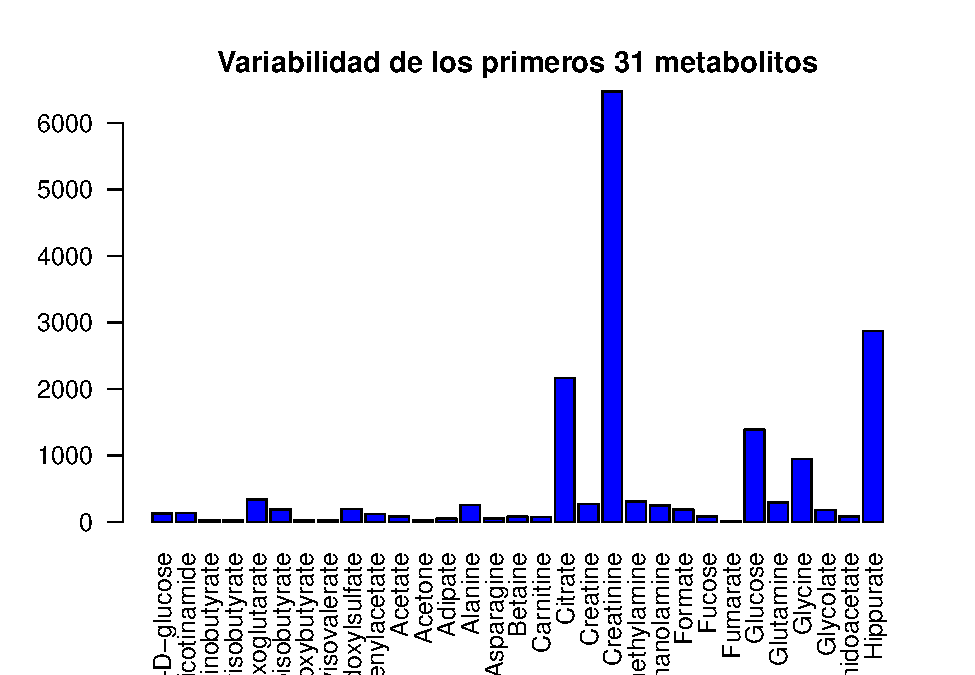
\includegraphics{PEC1_files/figure-latex/unnamed-chunk-8-1.pdf}

\begin{Shaded}
\begin{Highlighting}[]
\CommentTok{\# Graficar diagrama de barras de la variabilidad de los ultimos 32 metabolitos}
\FunctionTok{barplot}\NormalTok{(}\FunctionTok{tail}\NormalTok{(variabilidad,}\SpecialCharTok{{-}}\DecValTok{32}\NormalTok{), }\AttributeTok{main=}\StringTok{"Variabilidad de los ultimos 32 metabolitos"}\NormalTok{, }\AttributeTok{col=}\StringTok{"blue"}\NormalTok{, }\AttributeTok{las=}\DecValTok{2}\NormalTok{, }\AttributeTok{ylim=}\FunctionTok{c}\NormalTok{(}\DecValTok{0}\NormalTok{,}\DecValTok{6000}\NormalTok{))}
\end{Highlighting}
\end{Shaded}

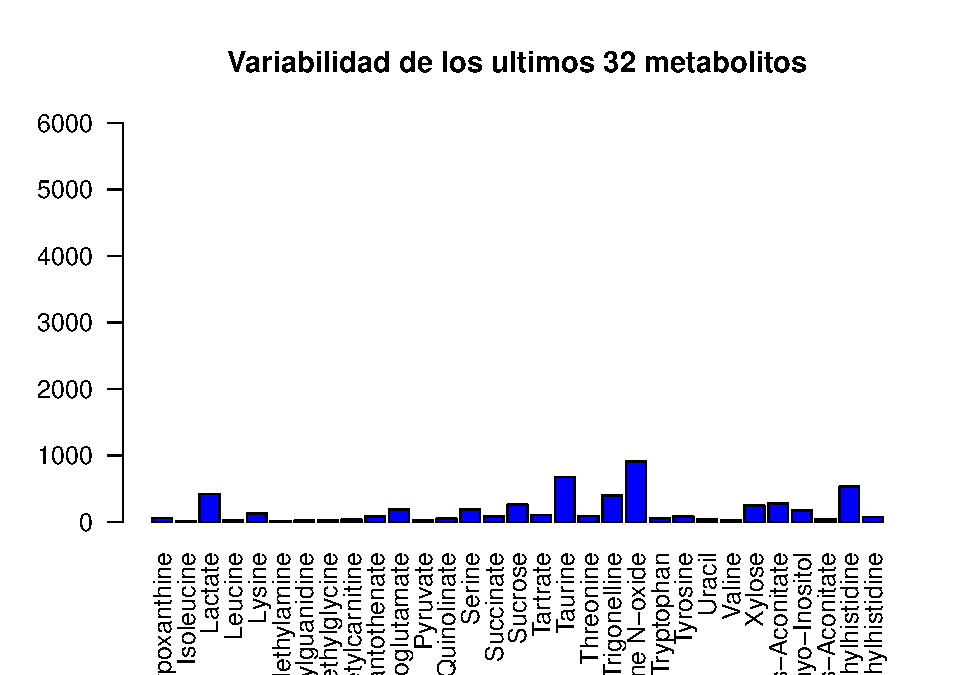
\includegraphics{PEC1_files/figure-latex/unnamed-chunk-8-2.pdf}

\subsection{Mapa de calor de los metabolitos y
muestras}\label{mapa-de-calor-de-los-metabolitos-y-muestras}

\begin{Shaded}
\begin{Highlighting}[]
\CommentTok{\# Instalar paquete}
\CommentTok{\# install.packages("pheatmap")}

\CommentTok{\# Llamar libreria}
\FunctionTok{library}\NormalTok{(pheatmap)}

\CommentTok{\# Normalizar los datos}
\NormalTok{data\_norm }\OtherTok{=} \FunctionTok{scale}\NormalTok{(}\FunctionTok{t}\NormalTok{(}\FunctionTok{assay}\NormalTok{(experimento)))}

\CommentTok{\# Obtener mapa de calor}
\FunctionTok{pheatmap}\NormalTok{(data\_norm, }\AttributeTok{main=}\StringTok{"Mapa de calor de los metabolitos y muestras"}\NormalTok{, }\AttributeTok{show\_rownames=}\ConstantTok{FALSE}\NormalTok{, }\AttributeTok{show\_colnames=}\ConstantTok{FALSE}\NormalTok{)}
\end{Highlighting}
\end{Shaded}

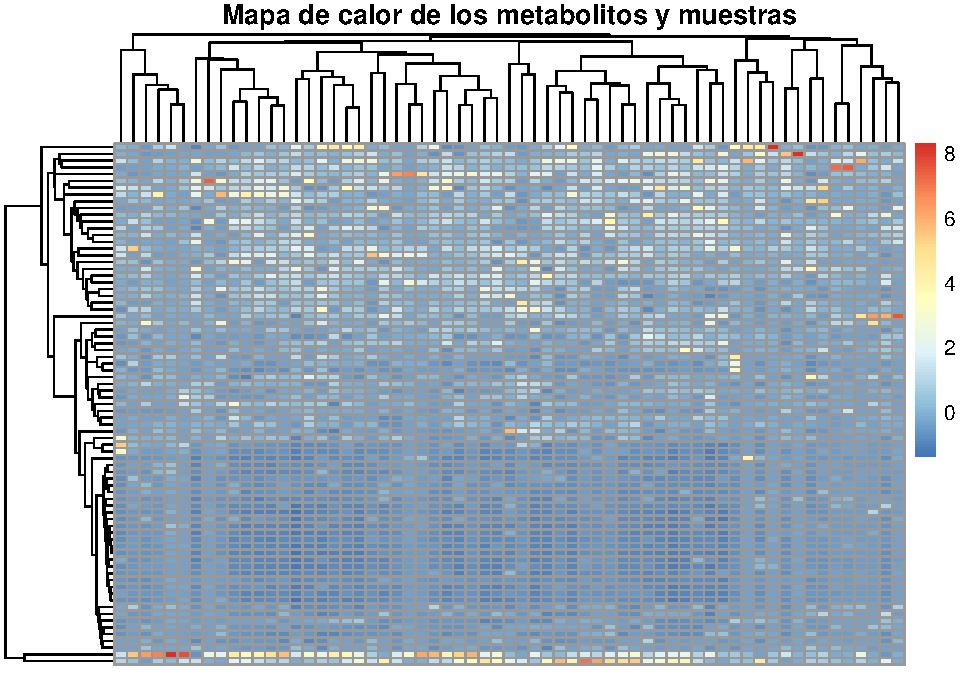
\includegraphics{PEC1_files/figure-latex/unnamed-chunk-9-1.pdf}

\subsection{Mapa de calor de la correlación entre los
metabolitos}\label{mapa-de-calor-de-la-correlaciuxf3n-entre-los-metabolitos}

\begin{Shaded}
\begin{Highlighting}[]
\CommentTok{\# Obtener la matriz de correlacion}
\NormalTok{cor\_matrix }\OtherTok{=} \FunctionTok{cor}\NormalTok{(}\FunctionTok{t}\NormalTok{(}\FunctionTok{assay}\NormalTok{(experimento)))}

\CommentTok{\# Crear mapa de calor de las correlaciones}
\FunctionTok{pheatmap}\NormalTok{(cor\_matrix, }\AttributeTok{main=}\StringTok{"Mapa de calor de correlación entre metabolitos"}\NormalTok{, }\AttributeTok{clustering\_distance\_rows=}\StringTok{"correlation"}\NormalTok{, }\AttributeTok{clustering\_distance\_cols=}\StringTok{"correlation"}\NormalTok{, , }\AttributeTok{show\_rownames=}\ConstantTok{FALSE}\NormalTok{, }\AttributeTok{show\_colnames=}\ConstantTok{FALSE}\NormalTok{)}
\end{Highlighting}
\end{Shaded}

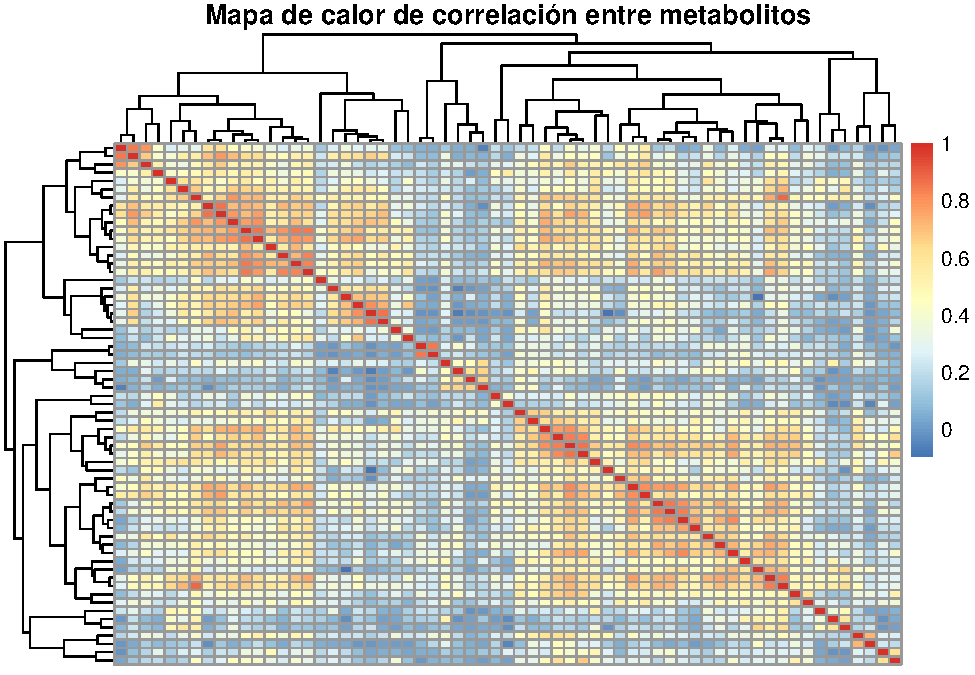
\includegraphics{PEC1_files/figure-latex/unnamed-chunk-10-1.pdf}

\subsection{Gráficas de los análisis de componentes
principales}\label{gruxe1ficas-de-los-anuxe1lisis-de-componentes-principales}

\begin{Shaded}
\begin{Highlighting}[]
\CommentTok{\# Llamar libreria}
\FunctionTok{library}\NormalTok{(ggplot2)}

\CommentTok{\# Obtener los grupos de muestras}
\NormalTok{grupos }\OtherTok{=} \FunctionTok{colData}\NormalTok{(experimento)}

\CommentTok{\# Realizar analisis de componentes principales}
\NormalTok{pca }\OtherTok{=} \FunctionTok{prcomp}\NormalTok{(}\FunctionTok{t}\NormalTok{(}\FunctionTok{assay}\NormalTok{(experimento)), }\AttributeTok{scale.=}\ConstantTok{TRUE}\NormalTok{)}

\CommentTok{\# Obtener datos del PCA en data frame}
\NormalTok{pca\_df }\OtherTok{=} \FunctionTok{data.frame}\NormalTok{(pca}\SpecialCharTok{$}\NormalTok{x)}

\CommentTok{\# Graficar PCA (primeros dos componentes)}
\NormalTok{p1 }\OtherTok{=} \FunctionTok{ggplot}\NormalTok{(pca\_df, }\FunctionTok{aes}\NormalTok{(PC1, PC2, }\AttributeTok{color=}\NormalTok{grupos}\SpecialCharTok{$}\NormalTok{grupo)) }\SpecialCharTok{+}
  \FunctionTok{geom\_point}\NormalTok{() }\SpecialCharTok{+}
  \FunctionTok{labs}\NormalTok{(}\AttributeTok{title=}\StringTok{"PCA de metabolitos y muestras"}\NormalTok{, }\AttributeTok{x=}\StringTok{"PC1"}\NormalTok{, }\AttributeTok{y=}\StringTok{"PC2"}\NormalTok{) }\SpecialCharTok{+}
  \FunctionTok{theme\_minimal}\NormalTok{()}
\CommentTok{\# Imprimir}
\FunctionTok{print}\NormalTok{(p1)}
\end{Highlighting}
\end{Shaded}

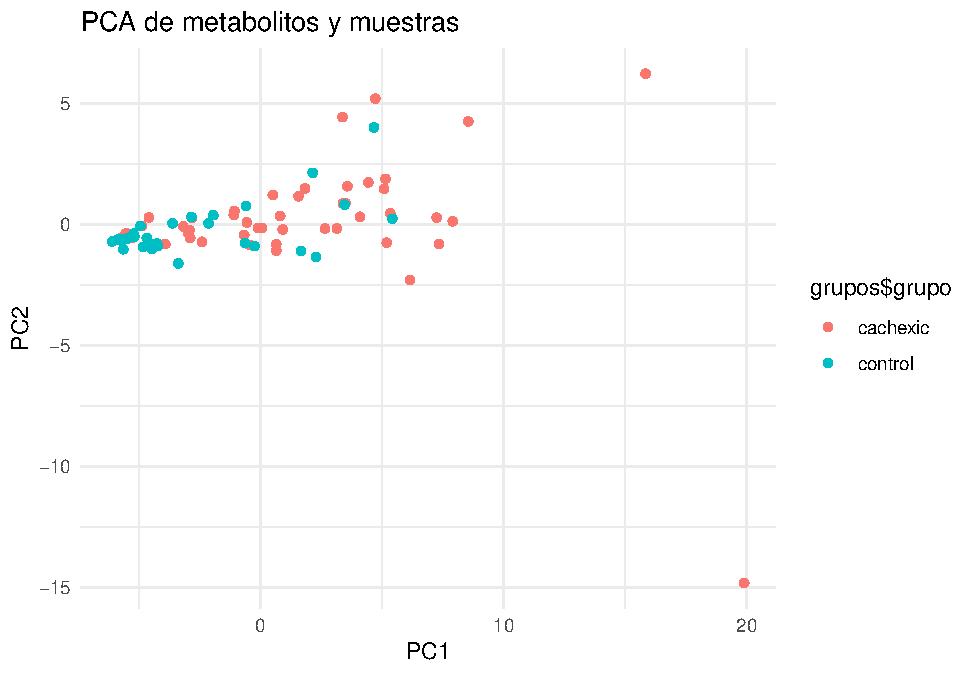
\includegraphics{PEC1_files/figure-latex/unnamed-chunk-11-1.pdf}

\begin{Shaded}
\begin{Highlighting}[]
\CommentTok{\# Graficar PCA (primero y tercer componente)}
\NormalTok{p2 }\OtherTok{=} \FunctionTok{ggplot}\NormalTok{(pca\_df, }\FunctionTok{aes}\NormalTok{(PC1, PC3, }\AttributeTok{color=}\NormalTok{grupos}\SpecialCharTok{$}\NormalTok{grupo)) }\SpecialCharTok{+}
  \FunctionTok{geom\_point}\NormalTok{() }\SpecialCharTok{+}
  \FunctionTok{labs}\NormalTok{(}\AttributeTok{title=}\StringTok{"PCA de metabolitos y muestras"}\NormalTok{, }\AttributeTok{x=}\StringTok{"PC1"}\NormalTok{, }\AttributeTok{y=}\StringTok{"PC3"}\NormalTok{) }\SpecialCharTok{+}
  \FunctionTok{theme\_minimal}\NormalTok{()}
\CommentTok{\# Imprimir}
\FunctionTok{print}\NormalTok{(p2)}
\end{Highlighting}
\end{Shaded}

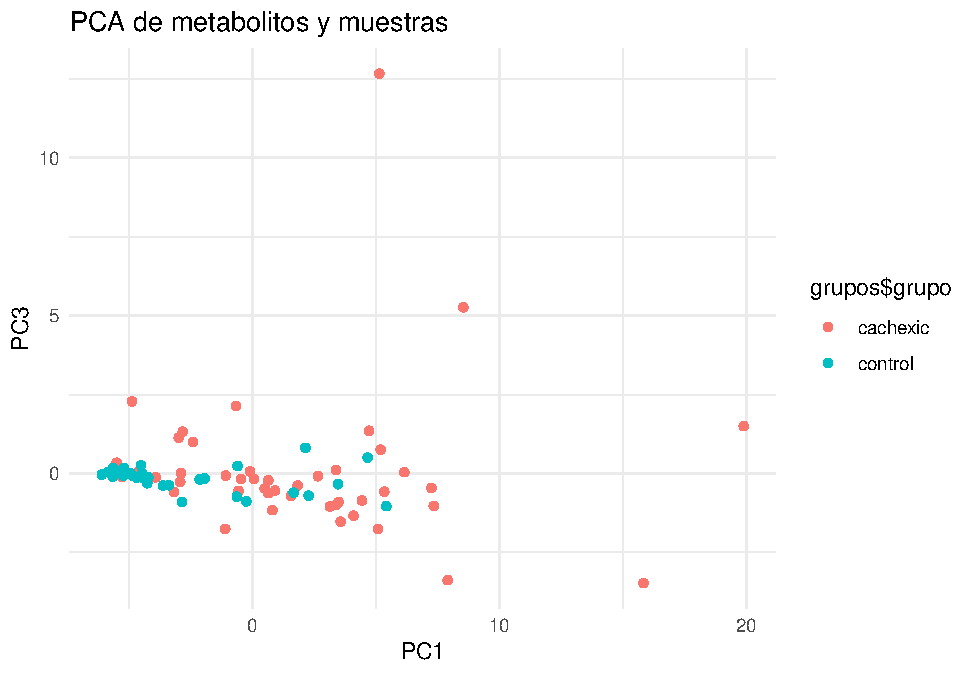
\includegraphics{PEC1_files/figure-latex/unnamed-chunk-11-2.pdf}

\begin{Shaded}
\begin{Highlighting}[]
\CommentTok{\# Graficar PCA (segundo y tercer componente)}
\NormalTok{p3 }\OtherTok{=} \FunctionTok{ggplot}\NormalTok{(pca\_df, }\FunctionTok{aes}\NormalTok{(PC2, PC3, }\AttributeTok{color=}\NormalTok{grupos}\SpecialCharTok{$}\NormalTok{grupo)) }\SpecialCharTok{+}
  \FunctionTok{geom\_point}\NormalTok{() }\SpecialCharTok{+}
  \FunctionTok{labs}\NormalTok{(}\AttributeTok{title=}\StringTok{"PCA de metabolitos y muestras"}\NormalTok{, }\AttributeTok{x=}\StringTok{"PC2"}\NormalTok{, }\AttributeTok{y=}\StringTok{"PC3"}\NormalTok{) }\SpecialCharTok{+}
  \FunctionTok{theme\_minimal}\NormalTok{()}
\CommentTok{\# Imprimir}
\FunctionTok{print}\NormalTok{(p3)}
\end{Highlighting}
\end{Shaded}

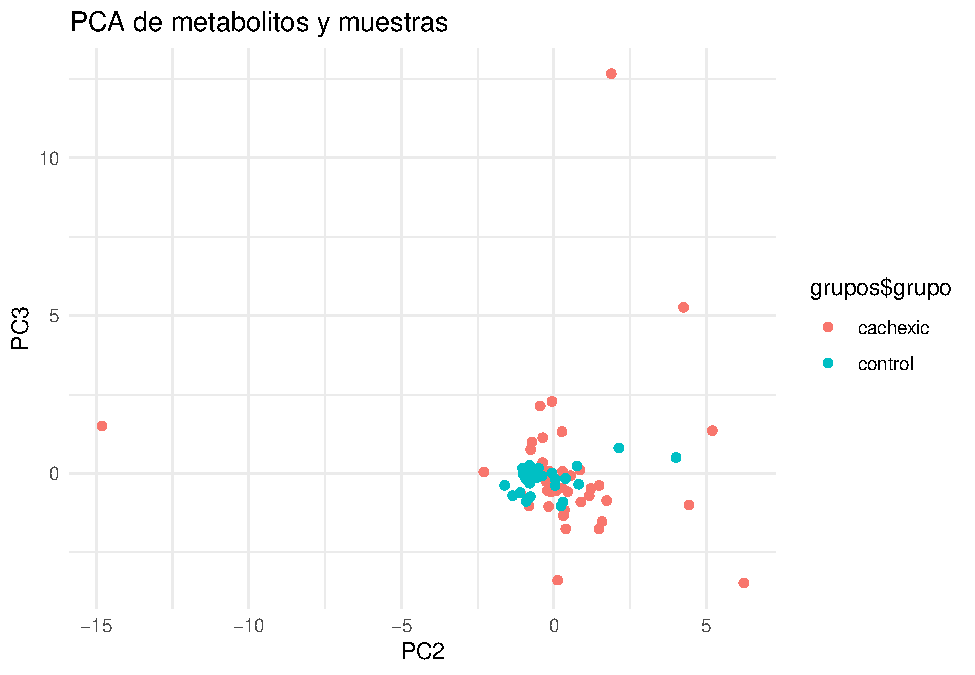
\includegraphics{PEC1_files/figure-latex/unnamed-chunk-11-3.pdf}

\begin{Shaded}
\begin{Highlighting}[]
\CommentTok{\# Obtener los nombres de los metabolitos}
\NormalTok{metabolitos }\OtherTok{=} \FunctionTok{rownames}\NormalTok{(}\FunctionTok{rowData}\NormalTok{(experimento))}

\CommentTok{\# Definir categorias de metabolitos}
\NormalTok{categorias }\OtherTok{=} \FunctionTok{list}\NormalTok{(}
  \StringTok{"Metabolismo de Carbohidratos"} \OtherTok{=} \FunctionTok{c}\NormalTok{(}\StringTok{"Glucose"}\NormalTok{, }\StringTok{"Pyruvate"}\NormalTok{, }\StringTok{"Lactate"}\NormalTok{, }\StringTok{"Acetate"}\NormalTok{, }\StringTok{"Citrate"}\NormalTok{, }\StringTok{"Fumarate"}\NormalTok{, }\StringTok{"Sucrose"}\NormalTok{, }\StringTok{"Xylose"}\NormalTok{, }\StringTok{"cis{-}Aconitate"}\NormalTok{, }\StringTok{"trans{-}Aconitate"}\NormalTok{),}
  
  \StringTok{"Metabolismo de Aminoacidos"} \OtherTok{=} \FunctionTok{c}\NormalTok{(}\StringTok{"Alanine"}\NormalTok{, }\StringTok{"Glutamine"}\NormalTok{, }\StringTok{"Glycine"}\NormalTok{, }\StringTok{"Serine"}\NormalTok{, }\StringTok{"Leucine"}\NormalTok{, }\StringTok{"Isoleucine"}\NormalTok{, }\StringTok{"Lysine"}\NormalTok{, }\StringTok{"Valine"}\NormalTok{, }\StringTok{"Threonine"}\NormalTok{, }\StringTok{"Histidine"}\NormalTok{, }\StringTok{"2{-}Aminobutyrate"}\NormalTok{, }\StringTok{"3{-}Aminoisobutyrate"}\NormalTok{, }\StringTok{"Guanidoacetate"}\NormalTok{, }\StringTok{"Methylguanidine"}\NormalTok{, }\StringTok{"Asparagine"}\NormalTok{, }\StringTok{"Betaine"}\NormalTok{, }\StringTok{"Ethanolamine"}\NormalTok{, }\StringTok{"Glycolate"}\NormalTok{, }\StringTok{"N,N{-}Dimethylglycine"}\NormalTok{, }\StringTok{"O{-}Acetylcarnitine"}\NormalTok{, }\StringTok{"Pyroglutamate"}\NormalTok{, }\StringTok{"Taurine"}\NormalTok{, }\StringTok{"Trigonelline"}\NormalTok{, }\StringTok{"Tryptophan"}\NormalTok{, }\StringTok{"Tyrosine"}\NormalTok{, }\StringTok{"pi{-}Methylhistidine"}\NormalTok{, }\StringTok{"tau{-}Methylhistidine"}\NormalTok{, }\StringTok{"2{-}Hydroxyisobutyrate"}\NormalTok{, }\StringTok{"3{-}Hydroxyisovalerate"}\NormalTok{),}
  
  \StringTok{"Metabolismo de Lipidos"} \OtherTok{=} \FunctionTok{c}\NormalTok{(}\StringTok{"Carnitine"}\NormalTok{, }\StringTok{"Acetone"}\NormalTok{, }\StringTok{"Adipate"}\NormalTok{, }\StringTok{"Trimethylamine N{-}oxide"}\NormalTok{),}
  
  \StringTok{"Metabolismo de Acidos Organicos y Ciclo de Krebs"} \OtherTok{=} \FunctionTok{c}\NormalTok{(}\StringTok{"Succinate"}\NormalTok{, }\StringTok{"Citrate"}\NormalTok{, }\StringTok{"Fumarate"}\NormalTok{, }\StringTok{"2{-}Oxoglutarate"}\NormalTok{, }\StringTok{"Acetate"}\NormalTok{, }\StringTok{"Acetone"}\NormalTok{, }\StringTok{"Formate"}\NormalTok{, }\StringTok{"Fucose"}\NormalTok{, }\StringTok{"cis{-}Aconitate"}\NormalTok{, }\StringTok{"trans{-}Aconitate"}\NormalTok{, }\StringTok{"Tartrate"}\NormalTok{),}
  
  \StringTok{"Metabolismo de Nucleotidos y Bases Nitrogenadas"} \OtherTok{=} \FunctionTok{c}\NormalTok{(}\StringTok{"Hypoxanthine"}\NormalTok{, }\StringTok{"Uracil"}\NormalTok{, }\StringTok{"Quinolinate"}\NormalTok{),}
  
  \StringTok{"Vias de Detoxificacion y Microbioma"} \OtherTok{=} \FunctionTok{c}\NormalTok{(}\StringTok{"Indoxyl sulfate"}\NormalTok{, }\StringTok{"Hippurate"}\NormalTok{, }\StringTok{"3{-}Indoxylsulfate"}\NormalTok{, }\StringTok{"4{-}Hydroxyphenylacetate"}\NormalTok{),}
  
  \StringTok{"Otras Vias Metabolicas"} \OtherTok{=} \FunctionTok{c}\NormalTok{(}\StringTok{"1,6{-}Anhydro{-}beta{-}D{-}glucose"}\NormalTok{, }\StringTok{"Dimethylamine"}\NormalTok{, }\StringTok{"Methylamine"}\NormalTok{, }\StringTok{"Pantothenate"}\NormalTok{, }\StringTok{"myo{-}Inositol"}\NormalTok{, }\StringTok{"1{-}Methylnicotinamide"}\NormalTok{),}
  
  \StringTok{"Biomarcadores de Estres y Energia"} \OtherTok{=} \FunctionTok{c}\NormalTok{(}\StringTok{"Creatine"}\NormalTok{, }\StringTok{"Creatinine"}\NormalTok{, }\StringTok{"3{-}Hydroxybutyrate"}\NormalTok{)}
\NormalTok{)}

\CommentTok{\# Encontrar la categoría correspondiente para cada metabolito}
\NormalTok{categoria\_df }\OtherTok{=} \FunctionTok{data.frame}\NormalTok{(}
  \AttributeTok{metabolito=}\NormalTok{metabolitos,}
  \AttributeTok{categoria=}\FunctionTok{sapply}\NormalTok{(metabolitos, }\ControlFlowTok{function}\NormalTok{(metabolito) \{}
\NormalTok{    category}\OtherTok{=}\ConstantTok{NA}
    \ControlFlowTok{for}\NormalTok{ (cat }\ControlFlowTok{in} \FunctionTok{names}\NormalTok{(categorias)) \{}
      \ControlFlowTok{if}\NormalTok{ (metabolito }\SpecialCharTok{\%in\%}\NormalTok{ categorias[[cat]]) \{}
\NormalTok{        category}\OtherTok{=}\NormalTok{cat}
        \ControlFlowTok{break}
\NormalTok{      \}}
\NormalTok{    \}}
    \FunctionTok{return}\NormalTok{(category)}
\NormalTok{  \})}
\NormalTok{)}

\CommentTok{\# Realizar analisis de componentes principales}
\NormalTok{pca\_metabolitos }\OtherTok{=} \FunctionTok{prcomp}\NormalTok{(}\FunctionTok{assay}\NormalTok{(experimento), }\AttributeTok{scale.=}\ConstantTok{TRUE}\NormalTok{)}

\CommentTok{\# Obtener datos del PCA en data frame}
\NormalTok{pca\_df\_metabolitos }\OtherTok{=} \FunctionTok{data.frame}\NormalTok{(pca\_metabolitos}\SpecialCharTok{$}\NormalTok{x)}

\CommentTok{\# Graficar PCA (primeros dos componentes)}
\NormalTok{p1 }\OtherTok{=} \FunctionTok{ggplot}\NormalTok{(pca\_df\_metabolitos, }\FunctionTok{aes}\NormalTok{(PC1, PC2, }\AttributeTok{color=}\NormalTok{categoria\_df}\SpecialCharTok{$}\NormalTok{categoria)) }\SpecialCharTok{+}
  \FunctionTok{geom\_point}\NormalTok{() }\SpecialCharTok{+}
  \FunctionTok{labs}\NormalTok{(}\AttributeTok{title=}\StringTok{"PCA de metabolitos y muestras"}\NormalTok{, }\AttributeTok{x=}\StringTok{"PC1"}\NormalTok{, }\AttributeTok{y=}\StringTok{"PC2"}\NormalTok{) }\SpecialCharTok{+}
  \FunctionTok{theme\_minimal}\NormalTok{()}
\CommentTok{\# Imprimir}
\FunctionTok{print}\NormalTok{(p1)}
\end{Highlighting}
\end{Shaded}

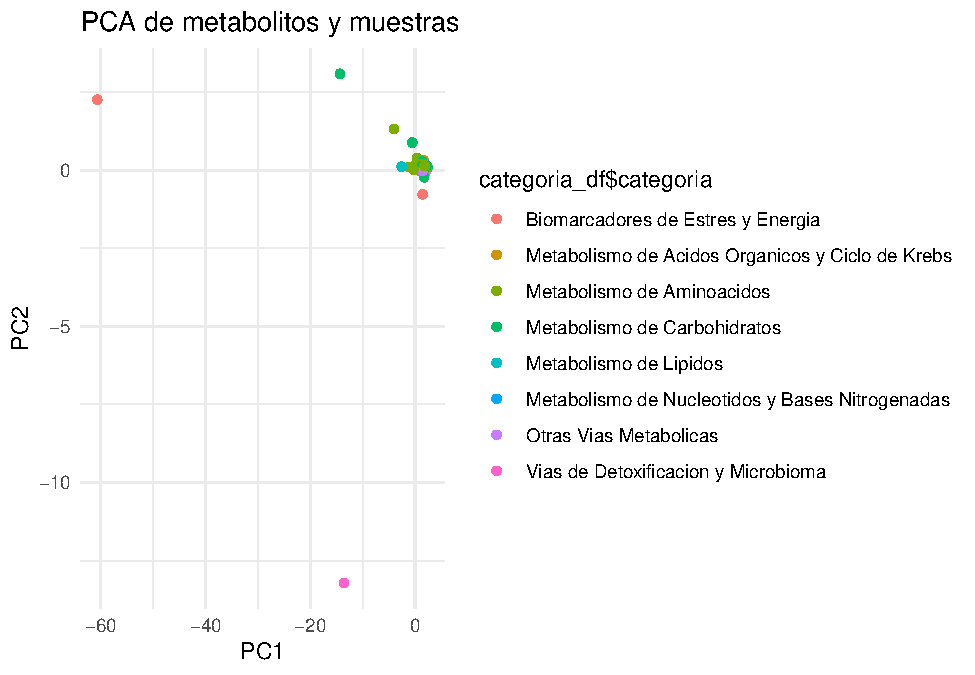
\includegraphics{PEC1_files/figure-latex/unnamed-chunk-11-4.pdf}

\begin{Shaded}
\begin{Highlighting}[]
\CommentTok{\# Graficar PCA (primer y tercer componente)}
\NormalTok{p2 }\OtherTok{=} \FunctionTok{ggplot}\NormalTok{(pca\_df\_metabolitos, }\FunctionTok{aes}\NormalTok{(PC1, PC3, }\AttributeTok{color=}\NormalTok{categoria\_df}\SpecialCharTok{$}\NormalTok{categoria)) }\SpecialCharTok{+}
  \FunctionTok{geom\_point}\NormalTok{() }\SpecialCharTok{+}
  \FunctionTok{labs}\NormalTok{(}\AttributeTok{title=}\StringTok{"PCA de metabolitos y muestras"}\NormalTok{, }\AttributeTok{x=}\StringTok{"PC1"}\NormalTok{, }\AttributeTok{y=}\StringTok{"PC3"}\NormalTok{) }\SpecialCharTok{+}
  \FunctionTok{theme\_minimal}\NormalTok{()}
\CommentTok{\# Imprimir}
\FunctionTok{print}\NormalTok{(p2)}
\end{Highlighting}
\end{Shaded}

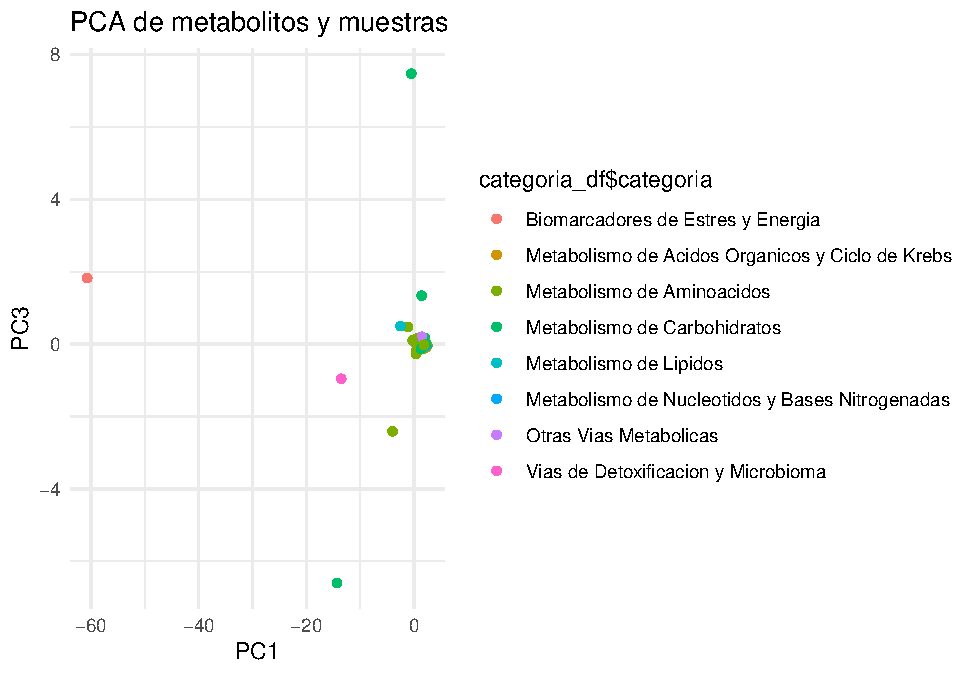
\includegraphics{PEC1_files/figure-latex/unnamed-chunk-11-5.pdf}

\begin{Shaded}
\begin{Highlighting}[]
\CommentTok{\# Graficar PCA (segundo y tercer componente)}
\NormalTok{p3 }\OtherTok{=} \FunctionTok{ggplot}\NormalTok{(pca\_df\_metabolitos, }\FunctionTok{aes}\NormalTok{(PC2, PC3, }\AttributeTok{color=}\NormalTok{categoria\_df}\SpecialCharTok{$}\NormalTok{categoria)) }\SpecialCharTok{+}
  \FunctionTok{geom\_point}\NormalTok{() }\SpecialCharTok{+}
  \FunctionTok{labs}\NormalTok{(}\AttributeTok{title=}\StringTok{"PCA de metabolitos y muestras"}\NormalTok{, }\AttributeTok{x=}\StringTok{"PC2"}\NormalTok{, }\AttributeTok{y=}\StringTok{"PC3"}\NormalTok{) }\SpecialCharTok{+}
  \FunctionTok{theme\_minimal}\NormalTok{()}
\CommentTok{\# Imprimir}
\FunctionTok{print}\NormalTok{(p3)}
\end{Highlighting}
\end{Shaded}

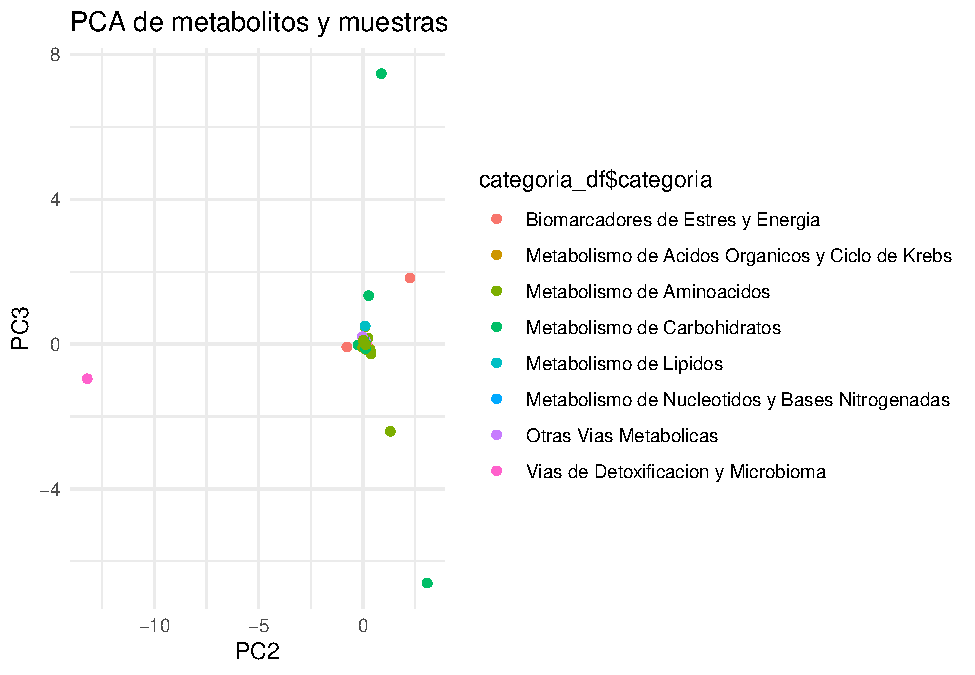
\includegraphics{PEC1_files/figure-latex/unnamed-chunk-11-6.pdf}

\end{document}
